%%%%%%%%%%%%%%%%%%%%%%%%%%%%%%%%%%%%%%%%%%%%%%%
%%%     Declarations (skip to Begin Document, line 88, for parts you fill in)
%%%%%%%%%%%%%%%%%%%%%%%%%%%%%%%%%%%%%%%%%%%%%%%

%%\documentclass[10pt]{article}
%%\documentclass[10pt]{report}
\documentclass[letterpaper]{article}
\usepackage{geometry}
%\usepackage{xcolor}
\usepackage[table]{xcolor}
\usepackage{amsmath}
\usepackage[some]{background}
%\usepackage{lipsum}
%\usepackage{natbib}
\usepackage[backend=biber, bibstyle=numeric, citestyle=numeric]{biblatex}  
%\usepackage{biblatex} 
\addbibresource{paperpile.bib}

%\usepackage{hyperref}

% Tables
\usepackage{float}
\usepackage[utf8]{inputenc}
\usepackage{tabularx}
\usepackage{booktabs}
\usepackage{longtable}

\usepackage{diagbox} %table split headers
\usepackage{longtable}
\usepackage{array}
\usepackage{rotating}
\usepackage{eqparbox}
\usepackage{makecell, caption, booktabs}

% Stuff needed to get table to span pages
\usepackage{enumitem}
%\usepackage{array, booktabs, longtable}
\newcolumntype{x}[1]{>{\raggedright}p{#1}}

\usepackage{etoolbox}
\AtBeginEnvironment{longtable}{%
    \setlist[itemize]{nosep,     % <-- new list setup
                      topsep     = 0pt       ,
                      partopsep  = 0pt       ,
                      leftmargin = *         ,
                      label      = $\bullet$ ,
                      before     = \vspace{-\baselineskip},
                      after      = \vspace{-0.5\baselineskip}
                        }
                           }% end of AtBeginEnvironment
% End table span
% Listings
\usepackage{listings}

\usepackage{geometry}  % Lots of layout options.  See http://en.wikibooks.org/wiki/LaTeX/Page_Layout
\geometry{letterpaper}  % ... or a4paper or a5paper or ... 
\usepackage{fullpage}  % somewhat standardized smaller margins (around an inch)
\usepackage{setspace}  % control line spacing in latex documents
\usepackage[parfill]{parskip}  % Activate to begin paragraphs with an empty line rather than an indent

\usepackage{amsmath,amssymb}  % latex math
\usepackage{empheq} % http://www.ctan.org/pkg/empheq
\usepackage{bm,upgreek}  % allows you to write bold greek letters (upper & lower case)

% for typsetting algorithm pseudocode see http://en.wikibooks.org/wiki/LaTeX/Algorithms_and_Pseudocode
\usepackage{algorithmic,algorithm}  

\usepackage{graphicx}  % inclusion of graphics; see: http://en.wikibooks.org/wiki/LaTeX/Importing_Graphics
% allow easy inclusion of .tif, .png graphics
\DeclareGraphicsRule{.tif}{png}{.png}{`convert #1 `dirname #1`/`basename #1 .tif`.png}

% \usepackage{subfigure}  % allows subfigures in figure
\usepackage{caption}
\usepackage{subcaption}

\usepackage{xspace}
\newcommand{\latex}{\LaTeX\xspace}

\usepackage{color}  % http://en.wikibooks.org/wiki/LaTeX/Colors

\long\def\todo#1{{\color{red}{\bf TODO: #1}}}

\long\def\ans#1{{\color{blue}{\em #1}}}
\long\def\ansnem#1{{\color{blue}#1}}
\long\def\boldred#1{{\color{red}{\bf #1}}}
\long\def\boldred#1{\textcolor{red}{\bf #1}}
\long\def\boldblue#1{\textcolor{blue}{\bf #1}}

% Useful package for syntax highlighting of specific code (such as python) -- see below
\usepackage{listings}  % http://en.wikibooks.org/wiki/LaTeX/Packages/Listings
\usepackage{textcomp}


%%% The following lines set up using the listings package
\renewcommand{\lstlistlistingname}{Code Listings}
\renewcommand{\lstlistingname}{Code Listing}

%%% Specific for python listings
\definecolor{gray}{gray}{0.5}
\definecolor{green}{rgb}{0,0.5,0}

\lstnewenvironment{python}[1][]{
\lstset{
language=python,
basicstyle=\footnotesize,  % could also use this -- a little larger \ttfamily\small\setstretch{1},
stringstyle=\color{red},
showstringspaces=false,
alsoletter={1234567890},
otherkeywords={\ , \}, \{},
keywordstyle=\color{blue},
emph={access,and,break,class,continue,def,del,elif ,else,%
except,exec,finally,for,from,global,if,import,in,i s,%
lambda,not,or,pass,print,raise,return,try,while},
emphstyle=\color{black}\bfseries,
emph={[2]True, False, None, self},
emphstyle=[2]\color{green},
emph={[3]from, import, as},
emphstyle=[3]\color{blue},
upquote=true,
morecomment=[s]{"""}{"""},
commentstyle=\color{gray}\slshape,
emph={[4]1, 2, 3, 4, 5, 6, 7, 8, 9, 0},
emphstyle=[4]\color{blue},
literate=*{:}{{\textcolor{blue}:}}{1}%
{=}{{\textcolor{blue}=}}{1}%
{-}{{\textcolor{blue}-}}{1}%
{+}{{\textcolor{blue}+}}{1}%
{*}{{\textcolor{blue}*}}{1}%
{!}{{\textcolor{blue}!}}{1}%
{(}{{\textcolor{blue}(}}{1}%
{)}{{\textcolor{blue})}}{1}%
{[}{{\textcolor{blue}[}}{1}%
{]}{{\textcolor{blue}]}}{1}%
{<}{{\textcolor{blue}<}}{1}%
{>}{{\textcolor{blue}>}}{1},%
%framexleftmargin=1mm, framextopmargin=1mm, frame=shadowbox, rulesepcolor=\color{blue},#1
framexleftmargin=1mm, framextopmargin=1mm, frame=single,#1
}}{}
%%% End python code listing definitions

\DeclareMathOperator{\diag}{diag}
\DeclareMathOperator{\cov}{cov}


%\bibliography{./paperpile.bib}
\author{Evan McGinnis}
\title{Automated Weeding}



\definecolor{titlepagecolor}{cmyk}{1,.60,0,.40}

\DeclareFixedFont{\bigsf}{T1}{phv}{b}{n}{1.5cm}

\backgroundsetup{
scale=1,
angle=0,
opacity=1,
contents={\begin{tikzpicture}[remember picture,overlay]
 \path [fill=titlepagecolor] (-0.5\paperwidth,5) rectangle (0.5\paperwidth,10);  
\end{tikzpicture}}
}
\makeatletter                       
\def\printauthor{%                  
    {\large \@author}}              
\makeatother
\author{%
    Evan McGinnis \\
    Graduate Student \\
    Biosystems Analytics \\
    \texttt{evanmc@email.arizona.edu}\vspace{40pt} \\
    }
\begin{document}
\begin{titlepage}
\BgThispage
\newgeometry{left=1cm,right=4cm}
\vspace*{1cm}
\noindent
%%\vspace*{0.4\textheight}
\textcolor{white}{\Huge\textbf{\textsf{Automated Weeding\\ in Lettuce Crop}}}
\vspace*{2.5cm}\par
\noindent
\begin{minipage}{0.35\linewidth}
    \begin{flushright}
        \printauthor
    \end{flushright}
\end{minipage} \hspace{15pt}
%
\begin{minipage}{0.02\linewidth}
    \rule{1pt}{175pt}
\end{minipage} \hspace{-10pt}
%
\begin{minipage}{0.6\linewidth}
\vspace{5pt}
    \begin{abstract} 
This paper presents a study of an automated weeding system for lettuce cultivars.  The system consists of two major subsystems, image processing and treatment. Of these two subsystems, only the image processing system is the subject of this study.
    \end{abstract}
\end{minipage}
\end{titlepage}
\restoregeometry
%
% F R O N T  M A T T E R
%
\tableofcontents
\listoffigures
\newpage

%
% O V E R V I E W 
%



\section{Introduction}

This document is intended as an overview of the work done to date on a project to automate the identification and treatment of unwanted vegetation in a field setting. This is not a proposal of work, so forward-looking statements are kept to a minimum (but might be sprinkled through this document) This is, however, a document that is continually revised, so while it is fairly close to current results, it may lag just a bit behind the current status.

The broad brush-strokes of the project are fairly simple:
The integrated system consists of three subsystems: image acquisition, image processor, and treatment system.
The system is towed behind a tractor in a field setting, and the system identifies and treats unwanted vegetation. (unwanted vegetation comes in two forms: weeds, and crop that should be thinned)

The treatment subsystem (a high-precision sprayer) has already been developed, and will not be discussed at length here)

\section{Literature Review}
Work in progress. Will be revised later

(Lin et al. 2017)
Has a PCA of reflectance using hyperspectral sensor.
Gives formulae for 4 different vegetation indices incorporating NIR and using reflectance at specific wavelengths.
Shape features considered: area, shape index, length/width, length, and texture. Shape index is the smoothness of an image object border.

Length/Width is the length-to-width ratio:




where eig1(S) is the maximum eigenvalue of the matrix S; eig2(S) is the minimum eigenvalue of the matrix S.

Texture is comparing the regularity of color distributions in plants  (monocots vs dicot vein structure is discussed) Using the gray level co-occurrence matrix (GLCM)


Assertions from this paper:
A combination of factors must be considered in weed discrimination (spectral reflectance, shape, texture

(Basavarajeshwari and Madhavanavar 2018)

This was a survey article leading to these references:

(Montalvo et al. 2016)
Details using PCA to improve vegetation indices.

(Raja et al. 2020)

Wirth, Michael. Lecture Slides

\section{Compute Environment}
These findings were executed on an HP Pavilion HPE Series Tower PC:
Intel I7 Processor with 4 Cores @ 3.4GHz
32GB RAM
Windows 10 Home
Logitech HD C920 webcam

The evaluation of timing data mentioned should bear this in mind. This machine was introduced in 2011. A more modern machine will, no doubt, have better performance. (Indeed, a modern high-end laptop has a CPU benchmark of 16168 in comparison with the author’s machine that is rated at 6367 -- a crude, but useful comparison.)

The author also has access to a recent macbook with these specifications:
Intel I5 Processor with 4 Cores @ 1.1Ghz
16GB RAM
macOS 11.3.1 (Big Sur)

\section{Test Data Preparation}
Test data comes in two forms: static images obtained with visible light cameras and prepared images of manually manipulated scenarios.

\subsection{Discrete Static Images}
Discrete image sets are those where there is likely to be a physical gap between adjacent images, so they must be processed without the context of adjoining neighbors. These images are useful for development and testing of weed identification by position and size, but is not very useful in situations that will be discussed in more detail in later sections of this document:
The identification of a crop row
The classification of vegetation not fully with the image.

The figure below demonstrates both of these issues. The crop row cannot be conclusively identified from the singled plant in the image (but can be assumed to be approximately in the middle of the image). The vegetation to the lower right hand side of the image cannot be conclusively identified as crop simply by position or size. In this case, the leaf is part of the plant that will appear in the neighboring image, but until we can see a larger portion of it, the imaging cannot be used for conclusive identification.


\subsection{Continuous Static Images}
Continuous image sets are those where neighbors are overlapping, lending themselves to a two step processing that results in evenly spaced images such that subsequent processing can consider adjacent images. It is perhaps easiest to consider the construction of a panoramic view of a city skyline. Multiple images, each overlapping its neighbor are stitched together by identification of common elements of both into a single panorama.

The development and verification of these images is accomplished by image capture of a continuous strip with distance markings. Photos of the strip are taken in a sequence and then reassembled into a continuous image. This continuous image is then broken apart into regularly spaced (or regularly overlapping) images. While it may seem a bit counterintuitive to stitch an image together only to then break it up, the point of this exercise is to simulate what a precisely timed imaging system would see. In that case, the imaging system would acquire images with exactly 20\% overlap, something not possible with manually acquired images. 

The images below illustrate this. The vertical strip below to the right of the carpet is taken in the author’s house.  The images to the right are two discrete images taken of the strip with  a generous amount overlap, at least 20\%. These images are then stitched together to form the panoramic image seen in Figure 3.


Figure 3. 
Unfortunately, the construction of a panoramic image from a series of  overlapping images is not as error-free as implied above. Forming a panorama from a dozen images may introduce color or geometric distortions that are not acceptable, and this appears to be exacerbated by the alignment between images.

Consider this image constructed by stitching together 11 manually acquired images:


Ignoring the banding above and below the image, the image contains distortions such as is shown below. This is in the same area as was distortion free when only two images were stitched. That is the key finding here: an image set acquired manually will almost never have the uniformity of alignment and framing required to produce a distortion free panorama across many images.



It is reasonable to stitch two adjacent images together, resulting in minimal distortion to address the case described above where vegetation at the edge of the image cannot be seen in its entirety.

These images are used to simulate a row of crop. Consider this image:

In this case, the green dots represent crop that is desired, and red dots undesirable weeds.
Much as we computed the vegetation index to segment the image into plants and background, we can segment out the dots by considering only those pixels containing green or red.  That is, we consider this another vegetation index algorithm we can add to the set already implemented. This results in the image below.




For the curious:  Using one of the other vegetation indices  (NGRDI) also picks up the blue painter’s tape.


\subsection{Prepared Images}
Single images are prepared using Adobe Photoshop to create test data for various scenarios:
Rows of vegetation requiring thinning
Unwanted vegetation too close to wanted vegetation
Debris in the image

Here, vegetation is placed within separate layers to create a composite image that shows the desired result. In this example, a single lettuce plant is replicated several times to form an image that appears to be that of several plants. Notice the obvious seam in the lettuce plant on the  right hand side of the image. As these pixels will be discarded early in image processing, they will have no effect on the current process as a whole, but may be a consideration if future processing considers factors such as the vegetation’s shadow.


\section{Calibration}
The primary parameter of interest in both static image sets and those obtained live from an attached camera is the number of pixels per mm. This will be used to estimate distances to objects detected in the image.  For both instances, the approach is the same:

Prepare a calibration target consisting of two colored dots whose centers are a specific distance apart.
Capture, or read in an image of the calibration target
Convert the image to HSV
Mask off any pixels that are not in the range of the color of the dots
Detect the dots and compute the centers
Determine the number of pixels between the dots and the value for pixels per mm for this image set.
Insert this value into a calibration file that will be used in subsequent processing

The figure below shows a calibration target with two green dots 3” apart (a pretty fancy description of a piece of paper taped to the floor with avery color code labels on it)

Figure 4. 

Steps 2-4 results in this image


Figure 5. 

This allows us to determine that the centers of the dots are 765 pixels apart in the example above. Knowing that the distance between centers is 76.2 mm gives a final value of 8.86 pixels per mm.

There are two key inputs to this system a user must provide: the color of the two dots (green, red, or blue) and how far apart those dots are in mm.

For example, this command line instructs the calibration utility: 
to read the image calibration.jpg, 
to write the results to calibrate.txt, 
that the dots are colored green, and 
that the dots are 76.2 mm apart.

%C:\weeds>python calibrate.py -i calibration.jpg -o calibrate.txt -c green -d 76.2

Under field conditions, it is anticipated that there would be a calibration phase before the system begins operation. This is probably no more complicated than placing a calibration target on the ground and executing the utility described above. Pragmatically, this process must be run only once, or whenever the distance between the image sensor and the ground is altered.
Work left to be done
This seems to be highly dependent on lighting conditions, so images read from my desktop webcam can’t be easily used for image processing in that the detection of the dots will fail unless they are quite brightly lit. The basic approach has been shown to work with static images, so getting this to work with the dynamic acquisition of images is an exercise for later.



It is not yet clear if color calibration is important to correct color imaging in a variety of lighting conditions, but as it is anticipated that lighting under field conditions will be tightly controlled, this step may not be required.

\section{Physical System}
The physical system components are as shown in this diagram.



Here, all components are connected by Cat6 Ethernet cables (solid lines), serial cables (wide arrows), or wireless (lightning bolt). The diagram demonstrates the devices and connectivity for a single bed, two crop line application, but the arrangement can be extended to cover additional beds. Such arrangements will not be addressed with specifics here, but such arrangements will be taken into account, such that the overall system is not specifically limited to the system detailed above.

Taking a look at each of these components
\subsection{Emitter}
The emitter will not be covered in any detail in this document, and is assumed to be a fully debugged subsystem that the system here can use.  The system here also makes a few assumptions about this system:
There are 6 treatment heads arranged as a linear array
Each treatment head can be individually opened or closed by applying or removing a +5V signal
The emitters are close enough to the application target that factoring the speed of the tractor in considering when an emitter is opened is not required.
The emitters operate in an enclosure such that it is not necessary to factor in wind or particle drift
The emitters can open and close fast enough that considering it in forming the treatment plan in not required
National Instruments cRIO
The National Instruments RIO model 9053 is described in this datasheet, and referenced in this document simply as “the RIO”. For the system described in this paper the RIO is powered by the factory supplied power adapter, best suited for desktop work (110 AC in via a standard 3 prong plug, XXX V DC out). Other power options are described in this article, but a supply suitable for field deployment is not considered here.
 
There are two interface cards of interest here:
9411, described in this datasheet
9403, described in this datasheet

Referencing the diagram above we can see two sets of devices connected to the controller via these: the rotary encoder and the emitter arrays. The RIO can accommodate 4 cards -- as we will see below, this will limit the number of emitter arrays to 12 (3 cards * 4 emitters per card) plus a single card for the rotary encoder.

NI 9411
The 9411 is connected to the rotary encoder via these pins: 1, 2, and 3 (corresponding to the A, B, and Z signals that will be discussed in the rotary encoder section).  While the voltage supplied by the card can power a +5V encoder, the model discussed in this document is a +10V model, so the outputs shown in the pinout diagram can be ignored for now. This assumption will be revisited when we consider an encoder requiring +5V.



NI 9403
The 9403 is connected to the emitter arrays. The pins on the 9403 are assigned to either array 1 or array 2 according to this scheme:



P0.1 - P0.6 Emitter array 1
P0.16 - P0.22 Emitter array 2

For prototyping,the pins are wired to an LED array as shown here to simulate the opening and closing of an emitter within an array:


\subsection{Rotary Encoder}
Distance is measured with a rotary encoder attached to a trailing wheel.

The specifics of the model TRD-GK1000-RZD used here are described in this datasheet

The encoder is wired to the RIO via this scheme:

The encoder is powered by a stand-alone power supply (standard outlet 2 prong 110V in, +12V 1 amp out) As discussed in the RIO section, an encoder with a lower power requirement can obviate the need for this component.

The rotary encoder is attached to the hub of this wheel (here, mounted on a benchtop)



The tape measure attached to the wheel is not required for field deployment and is used only for benchtop work to give a rough approximation of distance travelled.

The wires from the encoder, the power supply, and the cable attached to the RIO are wired with the scheme shown below.  The A/B/Z wires (black/white/orange) are connected to pins 1/2/3 on the connector. The power supply lines are routed through the connector only for neatness and do not connect to any pins, but to the brown wire directly. 

The connector referenced in this diagram is available here and the straight-through cable is available here.


This picture shows the final assembled cable.  The left hand side of the photo shows the encoder side, the top line feeding into the connector is from the power supply, and the right hand side of the photo shows the cable leading to the RIO.


\subsection{Nvidia Jetson Nano}

The Nvidia Jetson is described here is a 4GB Nano developer kit, suitable for benchtop and prototype solutions, but is not rugged enough for extended field trials. The development kit will be protected by housing it in a metal enclosure. The development kit is powered by a standalone power supply (standard outlet, 110 AC to DC 5V/4A).

Directly interacting with the Nano requires the use of a USB keyboard, USB mouse, and a HDMI monitor, however this will not be required for field deployment. That configuration is referred to as headless mode in the Nvidia literature.

For deployment, it is anticipated that the Nano developer kit will be replaced by a product suitable for field deployment, such as supplied by supplied by a solutions partner.  An example of this would be a Nano or Xavier system. (Rated to +70C operating temperature)

Persistent storage of the OS and code will be provided by this flash card, providing 128GB of storage.  This guide provides the instructions for the initial setup of the file system.
1Gb Ethernet POE+ switch
The 1Gbps ethernet switch connecting these components must have a minimum of 5 ports in the configuration outlined here. For the benchtop development, a simple 5 port switch was used capable of supplying POE for the devices that require it (specifications)  This switch is not rated for field conditions, as it rated for a +40C operating environment. The switch is powered by the included power supply (standard plug 110 AC to 48V DC/1.25A)
Basler Camera
The Basler Camera 1920-25ge is not produced by its manufacturer at this time, so detailed specifications are not included here.  This device is powered by the ethernet cable to the switch detailed in a previous section.

The lens attached to the Basler camera appears to be a Computar H0514-MP2, a 5mm focal length lens for a ½” sensor described here. Given the small sensor size supported by this lens, it is anticipated that a new one will be specified if a higher resolution camera is used.

Protection for the camera by means of a housing is probably a requirement to avoid damage and adverse environmental conditions (dust, chemicals), but is not yet considered or specified.
LED Lighting
The LED lighting is not yet specified, so details will not be provided here. The LEDs supply all illumination for the camera, as the entire system is contained within an enclosure that will block nearly all ambient light.
Wifi AP
The WiFi access point is not yet specified, so details will not be provided here. This is how external consoles will communicate with and control the system.  A rule of thumb here is that a WiFi signal can provide coverage to devices within 100 meters, enough for both ground observers and a tractor mount option.
Console
There are two consoles in this system (the specific number, as we will see, is not particularly important -- this could be greater than two): an operator’s console and that of a ground observer.  These distinctions may seem somewhat arbitrary, but each will be geared toward the roles each operator is expected to fill. A ground operator will concentrate on details of what the system is doing, whereas a tractor operator is concerned with operational control of the system (turning it on/off, monitoring for faults,etc.) Each console will be geared toward simple, touch screen interaction suitable for field use (few, large buttons, large text, etc.).

As we will see in the discussion of the software, there will also be a mechanism by which a laptop resident application will be used, but that is not considered to be a part of the system detailed here.

\subsection{Power Requirements}
Benchtop Development Environment
Most hardware elements detailed above are assembled into a working environment as illustrated here:


Most of these components are simply on (RIO, Jetson, Ethernet Switch) or -- as we saw previously --  mounted to the benchtop (encoder wheel).  The camera and LED lighting is mounted on a structure that approximates (as far as is practical) the conditions that will be encountered when installed in the field enclosure. The LED array is a stand-in for the emitter arrays, illuminating when supplied power from a corresponding pin.

In this structure (constructed from extruded aluminum, connectors, and gantry plates), the camera is mounted such that the distance between the front of the lens and the bottom of the structure is equal to what can be expected in the field enclosure (about 43 cm)




The camera can be moved back and forth, as it is mounted on a gantry plate with wheels that ride within the channels of the aluminum rail.  While difficult to see in the photo above, a flexible, metal tape measure is attached to the LED lighting to measure distance.

Note: the structure does not yet contain side and top panels to reproduce the field enclosure. This is planned, but will be a later addition.

\section{Software Development Environment}
The software described in this document was developed with these components
PyCharm Professional 2020.3 (Python IDE)
Python 3.8.5
OpenCV 4.x
Numpy
scikit-learn
Hashicorp Packer

The development was on an HP Pavilion HPE Series Tower PC:
Intel I7 Processor with 4 Cores @ 3.4GHz
32GB RAM
Windows 10 Home
Logitech HD C920 webcam

All software developed and discussed in this document can be obtained from this git repository:

https://github.com/evan-mcginnis/weeds

\section{Software System}
\section{Networking}

\section{Device Setup and Configuration}

\section{Device Diagnostics}

\section{Roles and Responsibilities}

\section{Inter-Device Communication}

\section{Basic Abstractions}
There are three basic abstractions used in this system to represent real-world objects:
\begin{itemize}
	\item{The odometer}
	\item{The camera}
	\item{The treatment array sprayer}
\end{itemize}

While much of the interaction between these components is beyond the scope of this document, it might be helpful to consider the roles and responsibilities of these objects in two forms: the manifestation of a physical system (i.e., an actual camera) and a purely virtual one (something the rest of the software believes to be a camera because it acts like one, but really just serves up images from disk.)

A camera can:
Take pictures
Run diagnostics
Give information about its capabilities such as resolution

An odometer can:
Call methods when it is detected that a specific distance has been travelled. In the physical world, an odometer might be a wheel that can be used to tell how far we have traveled.

The take-away from this is that hardware is just a detail.  For the purposes here it does not really matter to a system if a camera object represents a physical object that can take pictures or something that just serves up images from disk and can never actually acquire a new image. Hardware and the integration of that hardware is a very important detail, of course, but is not the sort of thing that prevents putting a basic system in place.


And a few more representing more components that don’t correspond neatly to real-world things...
The classifier, a component responsible for determining if vegetation is something desired or not. This component can make this determination using machine learning, neural networks, or heuristics. As with other components we have discussed, how it goes about this is of little concern to the rest of the system.
The treatment planner

An overly simplistic view of the flow between these objects is:



The image processor does not care if the odometer is backed by a device that can actually measure distance or if the odometer is simply something that makes calls at regular intervals and assumes a specific rate of travel.  All it does is to capture and process an image when instructed to do so. Likewise, the ImageProcessor is not dependent on the Camera representing an actual camera that can acquire images or something that claims to be a camera and when asked to take a picture simply returns one it read from disk.
Image Processing Flow
Acquire image
Computed Vegetation Index
Apply threshold to Index to create mask
Apply mask to image to isolate vegetation
Discover vegetation in images
Compute parameters of objects
Classify objects
\section{Approach To Classification}
The goal of this processing flow is to determine what each item within the image is and classify it as desired or undesired. Weeds are, of course, undesired, but crop plants can also be classified as undesired in the case of thinning operations. We will add a few designations to capture the situations we will encounter.
\begin{itemize}
	\item{Desired, the crop}
	\item{Undesired, either crop that must be thinned or weeds that can be treated without crop damage}
	\item{Unknown, vegetation that cannot be confidently identified}
	\item{Ignored, vegetation that is too close to desired vegetation to be treated without crop damage|
\end{itemize}

There are two basic approaches we can take:
\begin{itemize}
	\item{Identify the crop, and classify everything else as undesired}
	\item{Identify every item}
\end{itemize}

The techniques detailed in this document are geared more toward the first approach than the second. There are some simplifying assumptions we can make about the context of the images that will make crop identification a bit easier. Most importantly, identification of the crop line within the image is crucial to this approach, and is something that that will be discussed in greater detail in subsequent sections.
Vegetation Index

A vegetation index is applied to the images to produce segmentation between vegetation (something we care about) and soil/debris (something we don’t care about). The intent here is to reduce the information content of the image as a first step in image analysis. Soil and surface features of that soil represent noise we don’t want to process.

Here, we are using the Normalized Green Red Difference index, but the project has implementations for these algorithms, the details of which are beyond the scope of this document.

Normalized Difference Index
Excess Green
Excess Red
Color of Vegetation Extraction
Excess Green minus Excess Red
Normalized Green-Red Difference
Vegetative Index
Combined 1
Modified Excess Green
Combined 2
Triangular Greenness 


A visualization of NGRDI:



Row Detection
The initial attempts at crop row detection was through the us of a hough transform, and unfortunately, this had a few quirks that, while ultimately could probably be worked out:
Some images contained only a few, or in some cases a single plant along the crop row
The result of the transform was typically a set of lines in cases where the centers of the crop were not in perfect alignment.

To obtain exactly what is needed here, we make a few assumptions and follow a fairly simple methodology. Many of the proposals investigated are based on the more complex situation of identifying several crop rows in the same image. This instance, however, will encounter only a single crop row, greatly simplifying row detection.

Some assumptions:
The crop line is approximately in the middle of the image
Crop is typically in roughly horizontal alignment (the centers will be with a few degrees of each other)
Weed centers are typically not in horizontal alignment
There may be a single crop plant in the image or no crop at all

Leading to this method:
The distance to the center line of the image of each object is calculated
This distance is weighted by the area of each object
The object with the highest weighted distance is along the crop line.

The image below demonstrates a simple case. The green lines between centers show the angle between them. The exact center line of the image is labeled with a red line, and the computed crop line is rendered in green and labeled as such.


\section{Attributes of Vegetation in Image}
We have these attributes we can work with for objects detected in the image. The expectation here is that while no one feature can conclusively indicate that an object can be classified as as desired or undesired, the set of attributes can.

Position, especially relative to crop row
Size Ratio
Shape Index
Width/Length Ratio
Hue
Height
Position
Here the position of the vegetation relative to the crop row is weighted by the area of the vegetation. Consider this image:



Here, the unwanted vegetation (enclosed in a red bounding box) is assigned values above 0.4, whereas larger crop items along the crop lines are assigned values much closer to 0. (In this image, the vertical white lines from the center of vegetation to the crop line are simply for reference and have no significance)

Shape Index
Recall from a previous section that the shape index is a metric expressing the relationship between an object’s perimeter and its area:

When applied to objects in an image we see these values:



Width/Length Ratio

Recall from a previous section that the ratio width to length is given as




where eig1(S) is the maximum eigenvalue of the matrix S; eig2(S) is the minimum eigenvalue of the matrix S.

Colorspace Processing
Let’s consider two color spaces: HSV and HSI to see if hue can be a factor that can be used to differentiate weeds from crop. Consider this image:




An HSV visualization of this image demonstrates the Hue component as:

It is not clear from this display that the hue value of the weed is significantly different from that of the plant in this instance.

Converting the image to the HSI color space yields this visualization of the hue values, and once again it is not clear from this image that the hue of a weed differs from that of a crop.

This area certainly bears more investigation. This is an evaluation of only a single scene, but looking at an entire image set where we see a larger number of crop (type 0) and weed (type 1) the hue of a crop is fairly consistent, occupying a narrow band. 


It’s probably reasonable to assume that hue cannot be used as the sole criterion for distinguishing crop from weed, but if the hue is outside of the narrow band that the crop exhibits, it is more likely a weed than not.

It’s perhaps worth a moment to consider how these values were calculated.  Consider this plant enclosed in a bounding box:



For this calculation, we can consider this to be a rectangular matrix (the bit within the red boundary box). The black background is a don’t-care value and can be converted to Not-A-Number (NaN) such that when we calculate an average, only vegetated pixels are considered.

YIQ

Converting the image to the YIQ color space and examining the standard deviation of the I layer (the orange-blue data) yields this relationship indicating a fairly clear distinction between crop and weeds.



HSV

In the HSV colorspace, we can look at the average saturation values of the vegetation to yield this relationship indicating a fairly clear distinction between crop and weeds:



An interesting finding, but it remains to be seen if this relationship holds true for various stages in a development cycle.
Shape Analysis
Michael Wirth presents a summary of various techniques techniques for the shape analysis in this article. In depth analysis to evaluate the application of these techniques to these images has not yet been carried out, but these areas will be explored:
Compactness, the ratio of an object’s area to that of a circle
Elongation, the ratio of the width of a bounding box to its length
Eccentricity, the ratio of a minor axis to the major axis
Convexity, the relative amount an object differs from a convex object
Aspect ratio, the ratio of an object’s height to its width
Solidity, the density of an object, expressed as the ratio of an object’s area to its convex hull.
Radial distance measure, a measure of the boundary roughness.

The details of these techniques are conveniently missing here, but the idea here is to compute these metrics and use them as a part of the machine learning training set.

Height
This work is pending getting the size sensor working and taking field measurements with it. Discussions with technical support from the manufacturer are ongoing.

Performance
The time taken for various activities is shown in this table in processing a set of 38 images.








Row Labels
Average of milliseconds
Row Labels
acquire
142.2305366
acquire
angles
1.413414634
angles
classify
8.043780488
classify
contours
240.0440976
contours
hsi
728.1040488
hsi
hsv
23.57187805
hsv
index
212.1365366
index
LWRatio
2.437707317
LWRatio
mean
35.92956098
mean
overlap
0.048731707
overlap
shapes
0.146219512
shapes
stddev
46.3612439
stddev
treatment
3.753829268
treatment
ycc
21.47441463
ycc














Let’s look at the components that represent where a relatively large amount of time is spent and how (aside from code optimization) it can be improved.

Image Acquisition (140+ ms) This time represents the time taken from a virtual camera and is a measure of reading the image from disk. While this could be reduced to a millisecond or so if images were cached, this would not be encountered in the field, and is probably not worth optimizing. Under those conditions the system would access a physical camera, where image acquisition time is assumed to be (but is certainly not measured to be) a small number of milliseconds. This brings the total processing time down to around 579 ms, and is the value we will use in this analysis.
Contours (224+ ms) This is time taken up by the OpenCV library, a component that can use the GPU planned for field deployment.
Conversion to color spaces: HSI, HSV, YCC, and YIQ.  While HSI and YCC are acceptably small at around 20ms, conversion to YIQ and HSI at 188+ and 726+  are not. The  conversion to YIQ currently uses the scikit-image library, but this can probably made much faster with some matrix multiplication suitable for a numpy calculation, eliminating use of this library entirely.
Hue (36+ ms). This is a numpy calculation that can be optimized with a version of numpy that can use a GPU, CuPy: NumPy \& SciPy for GPU.
Vegetation Index (185+ ms) These are numpy calculations that can be optimized with the version mentioned in the previous step.


In general, it should be possible to move any manipulation of a matrix to a GPU. A reasonable time target for the processing of a single image is around 200 ms.

Readers should also note that these times represent entirely sequential processing. That is, the clock is started when the software first begins to process the image and stops when the treatment plan is calculated. In this case, however, a treatment plan can be calculated on the nth image while the system is processing the n+1th image -- parallel processing. The net effect of this is pretty much the same. The answer to the question of “how often can the system produce a treatment plan?” is unchanged. Here, it can be produced every 700ms. What parallel processing achieves, however, is that the system can execute other things at the same time as a treatment plan is formed and achieve the same throughput. While most attributes can be computed in parallel, the optimization achieved in doing so may not be worth the complexity cost, and will not substantively affect the answer to the question posed above.

The performance of the recognition system defines the maximum forward speed of the tractor. Here, we need to make an assumption, as we are working with an image set that is missing a few factors we need:
The horizontal length of an image is 600mm

Given this size, we can determine that the system can process an image in 600mm / 579 ms, or around 1.0363 mm/ms. Recall from a previous discussion that the target forward speed of the tractor is 1 meter/second, so we are just at the edge of what we want to achieve in terms of supported speed. The hand-waving bits of this analysis aside (the image acquisition time being reduced to zero is certainly suspect), this demonstrates that the system performance is at least in the ballpark of the values required.

Heuristic Classification
Before we start introducing techniques for classification using Machine Learning or Neural Networks, we need to first consider some basic heuristic techniques that can be applied to an image.  Consider these attributes of vegetation:
How far from the crop row is it?
What is the size of the vegetation in relation to other vegetation in the image?
Weed Detection using Size Elimination
Objects several times smaller than the largest object in the crop row are likely to be undesirable -- regardless of position with respect to the crop row. Consider this extract of a processed image:



In this instance, proximity to the cropline cannot be used as a criterion to determine that the vegetation is undesired. Indeed, it is closer to the cropline than other vegetation. Its area, however, is much smaller than that of other vegetation in the image: 10623 pixels for the plant near the center of the image vs 657712 pixels and 1002336.5 pixels for the neighbors to either side.
Based on this ratio, it is reasonable to determine that the vegetation is undesirable.
Classification using Machine Learning
To classify the objects within the image using machine learning, we first produce a dataset we can use to train the detector. In this case we can manually score each blob in an image.

Consider this image:



And this training data:



As a manual step, the vegetation names and types shown can be manually checked and altered, if required. Here we see that blob6 (the image name appears in the upper left hand corner) has been incorrectly identified as desired vegetation (type 0 -- that’s the column on the far right of the spreadsheet above). Once the training set has been manually scored, we are now ready to classify via machine learning algorithms.


Logistic Regression
Using some of the attributes detailed previously, we can apply logistic regression to predict the type of vegetation using a subset of the objects appearing in images acquired in the field.




(Ignore the name and number columns -- that’s just so I can relate this to decorated images)

The dataset excludes vegetation that cannot be fully seen in an image.

These are described in prior sections:
The Length/Width ratio
The shape index of the object
The distance from the crop line
The type of the vegetation: 1 = undesired, 0 = desired

Using this dataset split into 60/40 (training/testing) segments yields a model that is 96.5 % accurate in predicting the type of objects in the test set. However attempts to confirm this with R have hit a bit of a snag, as all coefficients are reporting as not significant

> summary(weedModel)

Call:
glm(formula = type ~ ratio + shape + distance, family = "binomial", 
    data = train, maxit = 100)

Deviance Residuals: 
       Min          1Q      Median          3Q         Max  
-9.615e-06   2.110e-08   2.110e-08   2.110e-08   1.229e-05  

Coefficients:
              Estimate Std. Error z value Pr(>|z|)
(Intercept)      79.43  508878.63   0.000        1
ratio           599.46 1173291.35   0.001        1
shape          -653.14 1278367.68  -0.001        1
distance         91.29  237156.90   0.000        1

(Dispersion parameter for binomial family taken to be 1)

    Null deviance: 9.5915e+01  on 125  degrees of freedom
Residual deviance: 3.4286e-10  on 122  degrees of freedom
AIC: 8


Removing the distance indication shows meaningful p values on the remaining factors:

> summary(weedModel)

Call:
glm(formula = type ~ ratio + shape, family = "binomial", data = train, 
    maxit = 100)

Deviance Residuals: 
    Min       1Q   Median       3Q      Max  
-1.6920   0.0000   0.0140   0.1009   3.4587  

Coefficients:
            Estimate Std. Error z value Pr(>|z|)    
(Intercept)    2.801      2.660   1.053 0.292343    
ratio          6.651      2.185   3.044 0.002335 ** 
shape         -8.129      2.138  -3.803 0.000143 ***
---
Signif. codes:  0 ‘***’ 0.001 ‘**’ 0.01 ‘*’ 0.05 ‘.’ 0.1 ‘ ’ 1

(Dispersion parameter for binomial family taken to be 1)

    Null deviance: 95.915  on 125  degrees of freedom
Residual deviance: 26.811  on 123  degrees of freedom
AIC: 32.811

Using a different package wish supports Firth's bias-Reduced penalized-likelihood logistic regression yields better results:

> weedModel2 <- logistf::logistf(formula = type ~ ratio + shape + distance, data = train)
> summary(weedModel2)
logistf::logistf(formula = type ~ ratio + shape + distance, data = train)

Model fitted by Penalized ML
Coefficients:
                  coef se(coef)   lower 0.95 upper 0.95     Chisq            p method
(Intercept)  0.8882576 2.558010  -4.36665548   6.177747  0.121010 7.279417e-01      2
ratio        5.5234812 1.961435   2.21126491  10.919413 23.225850 1.440480e-06      2
shape       -6.2814600 1.699084 -11.06455752  -3.422502 28.269870 1.055258e-07      2
distance     2.9874919 1.651566  -0.08123048   7.210671  3.625261 5.690864e-02      2

Method: 1-Wald, 2-Profile penalized log-likelihood, 3-None

Likelihood ratio test=64.33422 on 3 df, p=6.961098e-14, n=126
Wald test = 15.76606 on 3 df, p = 0.001266337
> 
> 




KNN
For classification with KNN, the number of neighbors was set to 1.
Random Forest
The number of estimators was set to 1000.
Decision Tree
No specific tuning parameters were applied.
Boosted Gradient
The maximum depth was set to 4.

Summary of various machine learning algorithms
These are the results of the scoring of a basic 40/60 split of the data

Algorithm
Train
Test
Logistic Regression
0.988
0.952
KNN
1
0.9
Decision Tree
1
0.9
Random Forest
1
0.9
Gradient Boosted
1
0.944


Perhaps an easier way of evaluating these algorithms is in terms of errors.  Here, a false positive is the identification of crop as weed, and a false negative as the identification of weed as crop.   Manually evaluating 238 objects within the image sets used shows these results:


Algorithm
False +
False -
Logistic Regression
0
4
KNN
6
11
Decision Tree
1
1
Random Forest
2
0
Gradient Boosted
1
0


Forming a Treatment Plan
Once the centers of undesired vegetation are identified, we need to form a treatment plan for that vegetation that is suitable for treatment by a grid or line of emitters. The formation of the plan follows these steps:

Divide the entire image up into a grid where the cell size is set to an arbitrary value for now
For each cell within the bounding box of the undesirable vegetation, mark that cell as requiring treatment if 75% of the pixels there represent vegetation. (The value of 75% is completely arbitrary and may be changed in response to investigations)

Consider this identified weed:



As covered in previous sections, this single weed is identified as three separate weeds, but for the purposes of forming a treatment plan, this will have no effect. Following the logic described above, we have this treatment plan, where each cell identified in red indicates a target cell.




Problems
Overlapping Vegetation

Overlapping vegetation is problematic in the current processing flow in that it is detected as part of the adjoining vegetation.  Consider this portion of an image:



The object detection algorithms are based on shapes of binary images, leading to the case where a few leaves of the weed are incorrectly identified as part of the crop. In this case,some leaves are identified as separate plants and are marked as requiring treatment, but this may not be the case with a larger plant requiring treatment that happens to overlap with desired vegetation.



This affects not only the inclusion of weeds with crop, but the misidentification of several weeds as a single plant, as this image demonstrates.  The three plants in the image are identified as a single blob as the overlapping leaves of multiple plants makes it appear as one.



Weed Shapes and Color
There are two complications with the identification of weeds by considering shape.  Computation of the shape index of objects within the image are complicated by poor lighting requiring more pixel dilation to make the vegetation appear to be a single plant. This, in turn, distorts the computation of the shape index of the object. The color of portions of the weeds does not produce the isolation of the entire plant.

Consider this image of a purslane weed:
Notice that this image exhibits both of these problematic properties. The color of the stem is a shade of red that is not isolated by considering only a single threshold of the vegetation indices discussed earlier in this document. The leaves also shade the stems to such an extent that the color is even closer to that of the surrounding soil. This problem is not unique to purslane, but can be seen in other vegetation with significant amounts of red in stems such as redroot pigweed.




This image displays the result of applying an NGRDI index to the image. Note that the stem of the plant is not displayed at all.


Which leads to the misidentification of leaves as separate plants



Recall that the image is constructed by creating a mask from a threshold applied to to an index and then using that mask to isolate vegetation. In this case, however, we have two sets of thresholds, one to isolate the vegetation and one to isolate the stems, leading to this image where the stems are visible.



However, this image suffers from the same problem as before with the misidentification of leaf clusters as separate plants.  An examination of the binary image used for blob identification reveals why this is happening.   The leaves are not joined together, and are still detected as distinct shapes.




Increasing the number of pixel dilations addresses this, bringing down the number of detected shapes significantly.


While this would appear to be a clean solution, it does come at a cost. As this binary image shows, the shape of the vegetation has now been distorted to the point where shape indices of the objects do not adequately represent the actual shape of the object..



Lighting
Lighting presents a challenge in that overly bright or overly dark regions tend to distort the detected shape of an object. Consider this example where the detected shape is overlaid over the actual image. In this case, it seems likely that the sensor was unable to capture the dynamic range of the darkest to lightest portion of the image, leading to some pixels being clipped.



In this example, the shape is detected as much more irregular than it actually is, distorting calculations for the shape index. Here, that shape index is computed as 2.03, but the actual value is certainly smaller. While various manipulations of the image of pixel dilation and erosions would lead to smoother edges, these manipulations would also lead to distortions of shape index calculations.

Now consider this image taken under similar field conditions.  Here we see that lighting is improved somewhat and that the edges detected more closely match those of the vegetation, leading to a more realistic calculation of a shape index. 


Controlling the lighting in images so that objects are evenly illuminated and within the dynamic range of the sensor would address these problems

Summary of data

Proposed Workflow


Image reproduced from: (Sabzi et al. 2020)




Jetson setup

%Change jumper as described here to allow for barrel connector
%https://forums.developer.nvidia.com/t/power-supply-considerations-for-jetson-nano-developer-kit/71637
%
%Set the static IP address as described here
%https://forums.developer.nvidia.com/t/set-static-ip-on-jetson-nano/107774
%
%Edit /etc/default/networking -- set CONFIGURE_INTERFACES=NO
%Edit ./etc/network/interfaces and add interface as described here:
%
%Iface eth0
%Address 169.254.212.40
%Netmask 255.255.255.0
%Gateway 169.254.212.31

Encoder Wheel Setup

Encoders (automationdirect.com)

Cable Design







%
% E N D  O V E R V I E W 
%

%
% I N T R O D U C T I O N
%
\section{Introduction}
This paper is part of a larger effort to detect weeds in imagery gathered under field conditions and treat those weeds in real-time. More precisely, weed detection with an image must be complete with 100s of milliseconds to treat weeds at commercially viable speeds. While such concerns are beyond the scope of this paper, we will instead focus on selecting object parameters that result in the most accurate predictions of the classification of vegetation into one of two categories: weed or crop. It is of no concern what specific species of weed or crop cultivar -- all that is important here is a binary classification of weed or not weed.\\
The dataset examined in this paper was gathered in an agricultural research field in Yuma, Arizona by capturing images while walking beside a planting bed. The processing of this image set follows this procedure:
\begin{enumerate}
	\item{Segment images (remove pixels that are not vegetation)}
	\item{Label vegetation as weed or crop}
	\item{Extract various parameters from  vegetation images}
	\item{Evaluate signficance of parameters to assigned class}
	\item{Evaluate predictions with various models using selected parameters}
\end{enumerate}

There are two problems with this dataset:
\begin{enumerate}
	\item{Weeds are underrepresented given the number of usable crop images}
	\item{Crop images are cut off in the images (and images are not acquired such that they can be stitched together to reconstruct them) and cannot be processed using structural features}
\end{enumerate}

%
% I M A G E  S E G M E N T A T I O N
%
\section{Image Segmentation}
The portions of the images that did not contain pixels with vegetation present were discarded. These images were segmented using various visible light indices \cite{Wirth2004-li}. As this process is not the primary subject of this paper, it will be given only superficial mention here.  Various approaches to image segmentation are  summarized in Table \ref{fig:indices}.

% SPAN
\begin{longtable}{x{\dimexpr.2\columnwidth-2\tabcolsep}
                  x{\dimexpr.4\columnwidth-2\tabcolsep}
                  x{\dimexpr.4\columnwidth-2\tabcolsep}}
%\begin{hyphenrules}{nohyphenation}
    \caption{Visible light indices}\label{tab:example}  \\
\toprule
{\textbf{Index}} & {\textbf{Formula}} & {\textbf{Comment}}
\tabularnewline
\midrule
    \endfirsthead
%%%%
    \caption{Visible light indices (cont.)}\label{tab:example}  \\
\toprule
{\textbf{Index}} & {\textbf{Formula}} & {\textbf{Comment}}
\tabularnewline
\midrule
    \endhead
%%%%
\midrule[\heavyrulewidth]
\multicolumn{3}{r}{\footnotesize\itshape
                   Continued on the next page}
    \endfoot
%%%%
\bottomrule
    \endlastfoot
%%%%
		Triangular Greenness
		& \begin{minipage}[t]{0.3\textwidth}
			$R_{green} - \alpha R_{red} - \beta R_{blue}\\ \alpha = \frac {2(\lambda_{blue} - \lambda_{green})} {(\lambda_{blue} - \lambda_{red})}\\ 
		    	\beta = \frac {2(\lambda_{green} - \lambda_{red})} {(\lambda_{blue} - \lambda_{red})} $
		   \end{minipage}     
		& Corrects for camera calibration using the peak sensitivity
\tabularnewline\addlinespace

		Normalized Difference     
		& $128 * \left( \left( \frac {(G - R)} {(G + R)} \right) + 1 \right) $                    
		& The NDI index produces a near-binary image. 
\tabularnewline\addlinespace

		Excess Green      
		& \begin{minipage}[t]{0.3\textwidth}
			$R = \frac {R} {R_{max}}\\ G = \frac {G} {G_{max}}\\ B = \frac {B} {B_{max}}$ 
		   \end{minipage}
		& ExG provided a clear contrast between plants and soil 
\tabularnewline\addlinespace

		Excess Red      
		& $1.3 R - G$ 
		& inspired by the fact that there are 4\% blue, and 32\% green, compared with 64\% red cones in the retina of the human eye
\tabularnewline\addlinespace

		Color Index of Vegetation Extraction      
		& $0.441 R - 0.811 G + 0.385 B + 18.78745$
		& This method was proposed to separate green plants from soil background in order to evaluate the crop growing status.
\tabularnewline\addlinespace

		Excess Green - Excess Red   
		& $ExG - ExR$ 
		& ExG used to extract the plant region and ExR used to eliminate the background noise (soil and residue) where green–red material (stems, branches, or petioles) may exist
\tabularnewline\addlinespace

		Normalized Green-Red Difference    
		& $\frac {(G - R)} {(G + R)}$ 
		& The method of NGRDI was used to overcome the differences in exposure settings selected by the digital camera when acquiring aerial photography of the field. 
\tabularnewline\addlinespace

		Vegetative Index      
		& $\frac {G} {R^aB^{(1-a)}}, a = 0.667$ 
		& VEG has a significant advantage because it is robust to lighting change.
\tabularnewline\addlinespace

		Com1   
		& $ExG + CIVE + ExGR + VEG$ 
		& TODO
\tabularnewline\addlinespace

		Modified Excess Green      
		& $1.262G - 0.884R = 0.311B$ 
		& TODO 
\tabularnewline\addlinespace

		Combined Indices 2      
		& $0.36ExG + 0.47CIVE + 0.17VEG$ 
		& Uses weighting factors to emphasize strengths of various approaches
\tabularnewline\addlinespace

\tabularnewline\addlinespace
\end{longtable}
% SPAN
%
% T A B L E  O F  S E G M E N T A T I O N  F O R M U L A E
%
% A bit more space on the table rows, so everything does not look so cramped
{\renewcommand{\arraystretch}{2}%
\begin{table}[H]
%\begin{longtable}{ccc}
    \caption{Visible light indices (\cite{Hamuda2016-dw,Hunt2013-ih})}
    \label{fig:indices}
    \begin{tabular}{  l  p{4cm}  p{5cm} }
        \toprule
\textbf{Index}      
& \textbf{Formula}   
& \textbf{Comment} \\\midrule
Triangular Greeness
& \begin{minipage}[t]{0.3\textwidth}
	$R_{green} - \alpha R_{red} - \beta R_{blue}\\ \alpha = \frac {2(\lambda_{blue} - \lambda_{green})} {(\lambda_{blue} - \lambda_{red})}\\ 
    	\beta = \frac {2(\lambda_{green} - \lambda_{red})} {(\lambda_{blue} - \lambda_{red})} $
   \end{minipage}     
& Corrects for camera calibration using the peak sensitivity \\\hline
Normalized Difference     
& $128 * \left( \left( \frac {(G - R)} {(G + R)} \right) + 1 \right) $                    
& The NDI index produces a near-binary image.  \\\hline
Excess Green      
& \begin{minipage}[t]{0.3\textwidth}
	$R = \frac {R} {R_{max}}\\ G = \frac {G} {G_{max}}\\ B = \frac {B} {B_{max}}$ 
   \end{minipage}
& ExG provided a clear contrast between plants and soil \\\hline
Excess Red      
& $1.3 R - G$ 
& inspired by the fact that there are 4\% blue, and 32\% green, compared with 64\% red cones in the retina of the human eye \\\hline
Color Index of Vegetation Extraction      
& $0.441 R - 0.811 G + 0.385 B + 18.78745$
& This method was proposed to separate green plants from soil background in order to evaluate the crop growing status. \\\hline
Excess Green - Excess Red   
& $ExG - ExR$ 
& ExG used to extract the plant region and ExR used to eliminate the background noise (soil and residue) where green–red material (stems, branches, or petioles) may exist \\\hline
Normalized Green-Red Difference    
& $\frac {(G - R)} {(G + R)}$ 
& The method of NGRDI was used to overcome the differences in exposure settings selected by the digital camera when acquiring aerial photography of the field. \\\hline
Vegetative Index      
& $\frac {G} {R^aB^{(1-a)}}, a = 0.667$ 
& VEG has a significant advantage because it is robust to lighting change.\\\hline
Com1   
& $ExG + CIVE + ExGR + VEG$ 
& TODO \\\hline
Modified Excess Green      
& $1.262G - 0.884R = 0.311B$ 
& TODO \\\hline
Combined Indices 2      
& $0.36ExG + 0.47CIVE + 0.17VEG$ 
& Uses weighting factors to emphasize strengths of various approaches\\\hline    

        \bottomrule
    \end{tabular}
\end{table}
%\end{longtable}
These indices are used to create a mask that is then applied to the original source image to permit vegetation to show while masking details that are not relevant (ground pixels, stones, and other items that may appear in field conditions) The intent here is to remove all pixels that are not relavent to the task of distinguishing between crop and weed:\footnote{Observers will note that the segmentation photo is rotated. This bears further investigation, but will have no impact on the features examined here.}
\begin{figure}[H]
\centering
\begin{subfigure}[]{.32\textwidth}
  \centering
  \includegraphics[width=1\linewidth]{figures/before-segmentation.jpg}
  \caption{Field view of lettuce and weed}
  \label{fig:sub1}
\end{subfigure}
\begin{subfigure}{.32\textwidth}
  \centering
  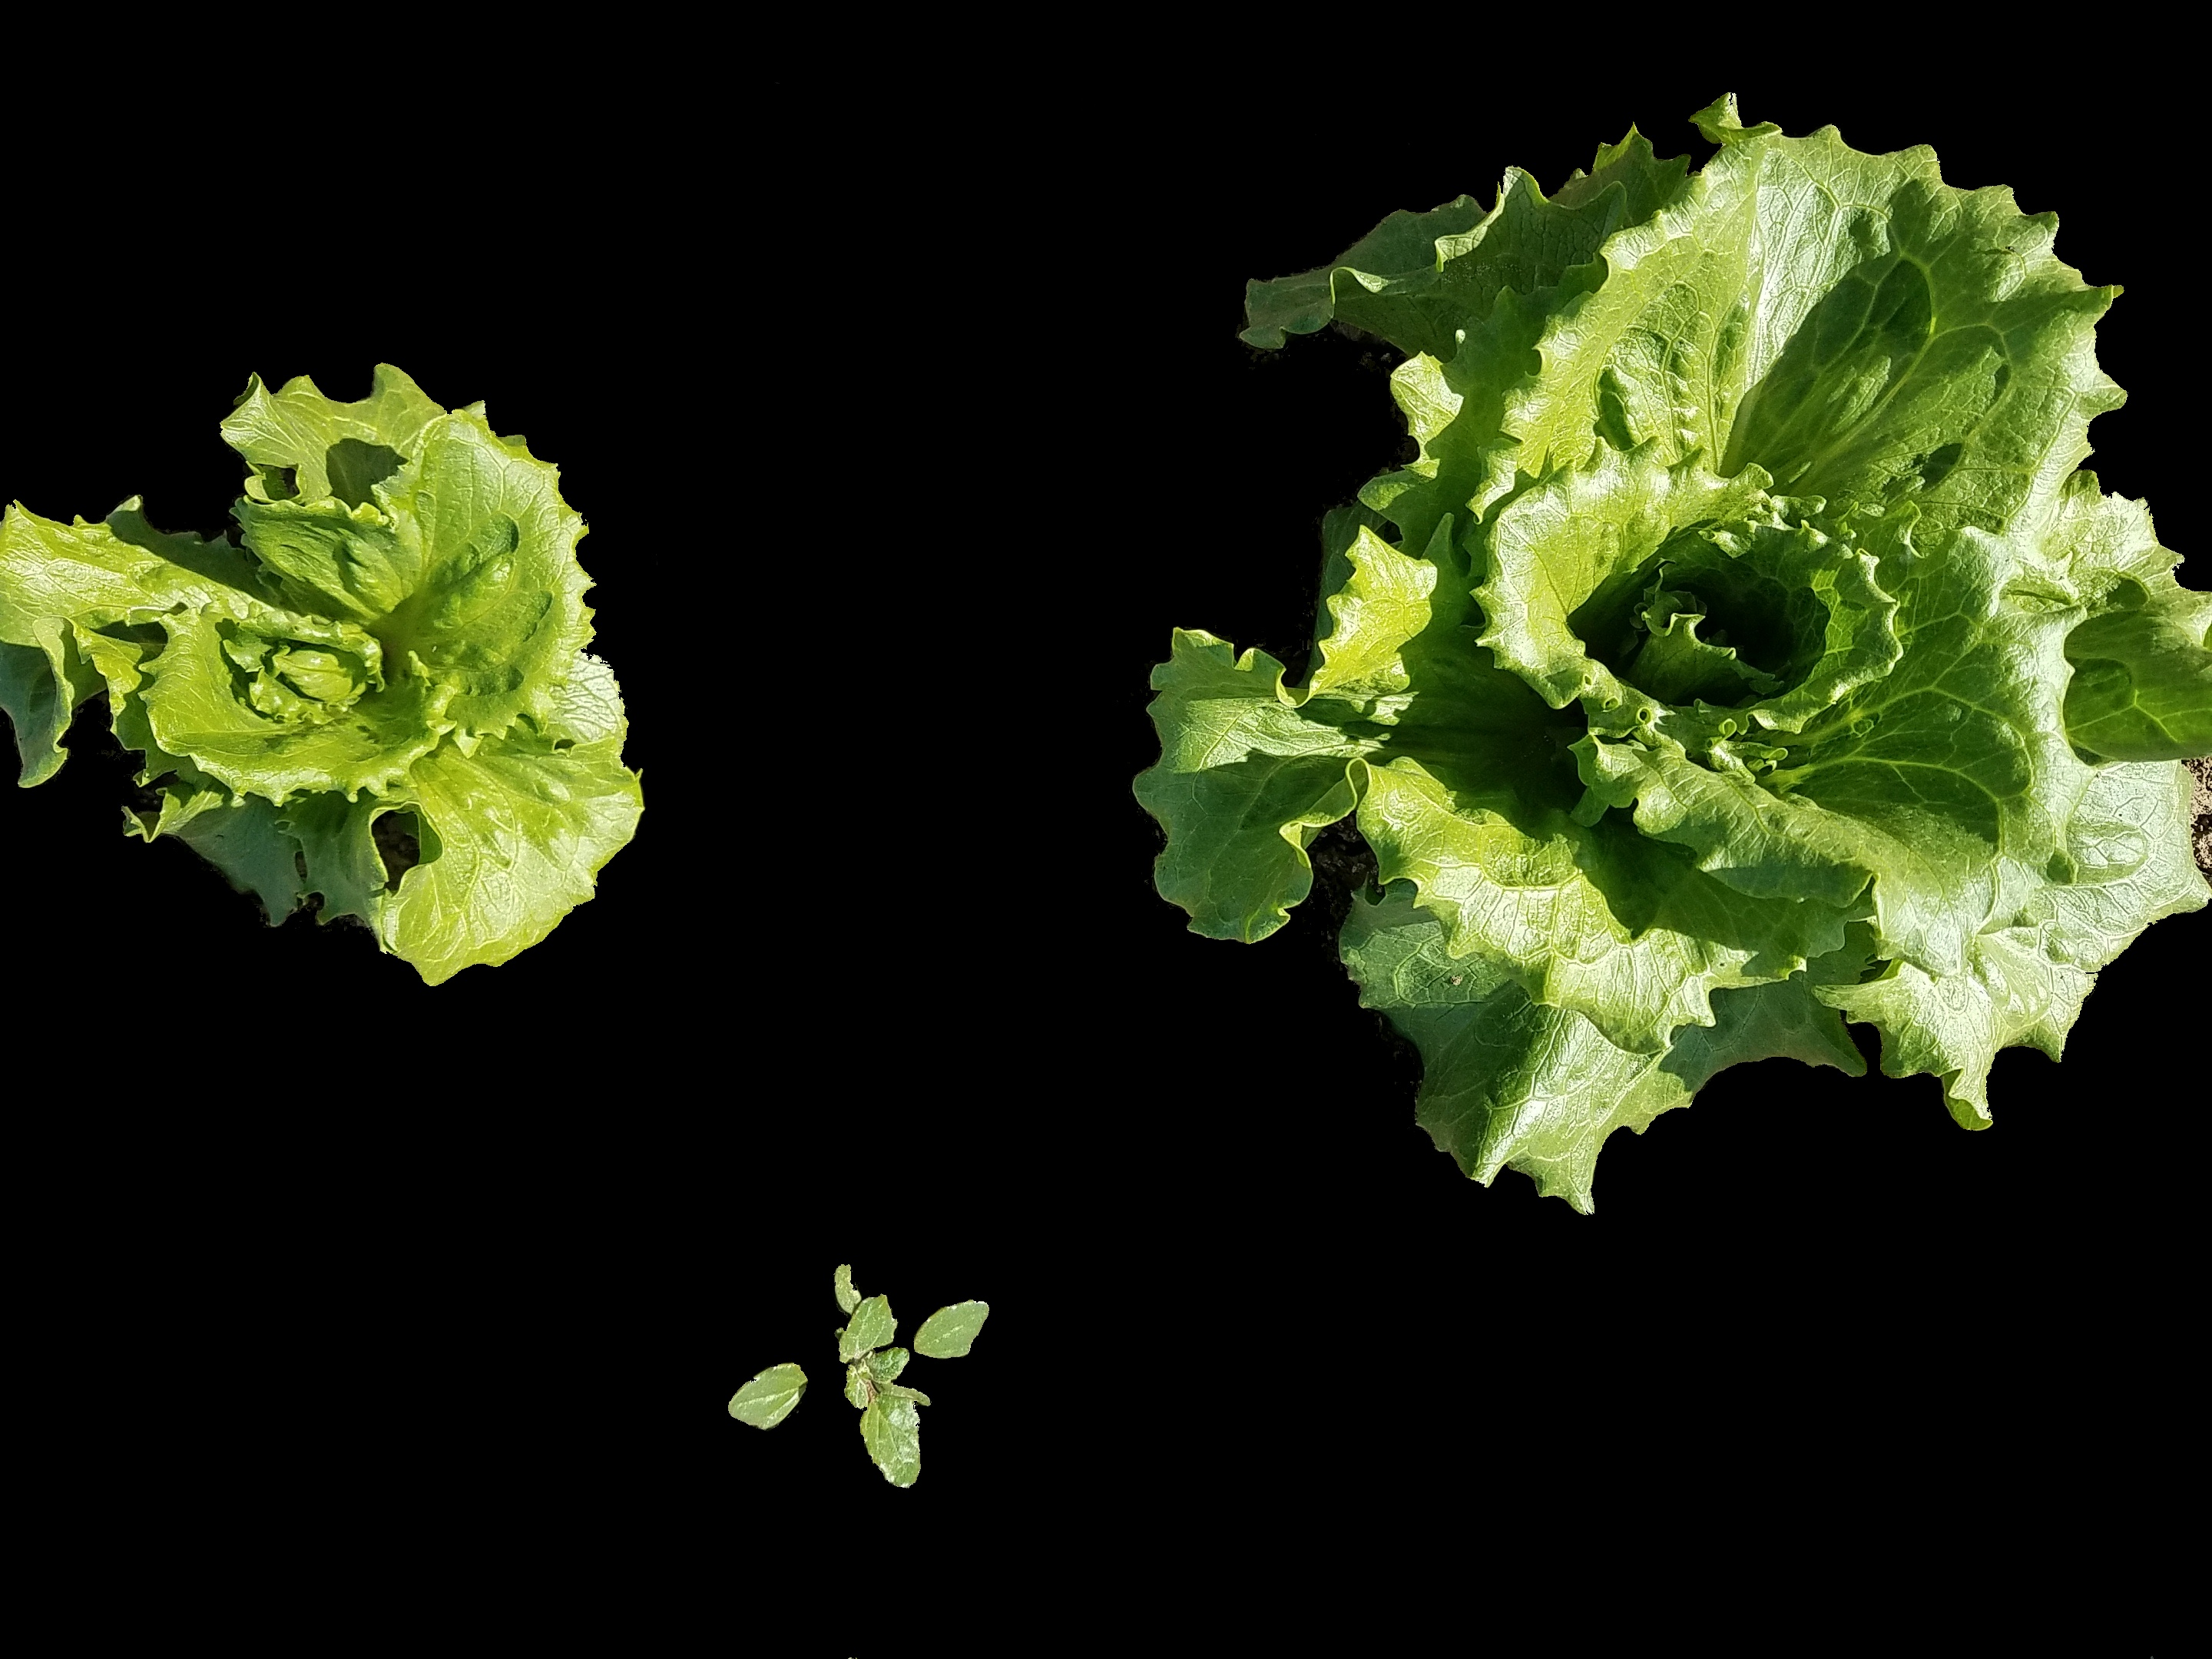
\includegraphics[width=1\linewidth]{figures/after-segmentation.jpg}
  \caption{After segmentation using NDI}
  \label{fig:sub2}
\end{subfigure}
\caption{Before and after segmentation}
\label{fig:segmentation}
\end{figure}
The segmented image has discarded ground pixels while retaining most of the pixels that will be used, but a close examination reveals that pixels in the stems of the weed are also eliminated, as they are less green than the rest of the plant. While they are not eliminated, pixels in the area of the deep shadows of the vegetation may affect attempts to classify objects based on color attributes. It is also envisioned that in the field images will be aquired under controlled, not ambient lighting conditions. For the purposes of this paper, images will use the NDI segmentation approach.


\section{Feature Extraction}
The library used for feature extraction is the OpenCV toolkit, so the discussion of various features may inadvertently slip into using OpenCV terms. Some basic shape descriptors are used below, and the most fundamental ones that apply here are the bounding box, the rectangular box that completely encloses the object, and the convex hull (and convex area), the smallest set of straight lines that completely contains an object. The concept of a {\it centroid} is also important to this discussion.  A centroid is the center of mass of an object, and a concept that will be used in this analysis.

The segmented images produced are then processed by a first identifying the separate objects (often called blobs) within the image and then computing various aspects of each of those objects. Weeds or crop may tend to exhibit these features to an extent that they can be used to distinquish between the two.  Weeds, for instance, may be more elongated than crop, or may tend to have saturation differences that may not be readily apparent to the casual observer.
\subsection{Length Width Ratio}
The ratio of width to length is not -- as the name might imply -- a simple ratio, but is expressed as:
\begin{eqnarray*}
S = 
	\begin{bmatrix}
	Var(X) & Cov(XY) \\[0.3em]
	Cov(XY) & Var(Y) \\[0.3em]
	\end{bmatrix},
\lambda = \frac {eig_{1}(S)} {eig_{2}(S)}
\end{eqnarray*}
Where $eig_{1}(S)$ and $eig_{2}(S)$ are the maximum eigenvalues of the matrix $S$, with $\lambda$ representing the ratio. \cite{Lin2017-xq}
\subsection{Shape Index}
The shape index of an object is a metric expressing the relationship between an object's perimeter and its area.
\begin{eqnarray*}
\alpha = \frac {e} {4 \sqrt{A}}
\end{eqnarray*}

\subsection{Normalized Distance from Cropline}
The cropline in a planting is, simply, the line along the bed where crop can be expected. Under field conditions the cropline will appear in the same spot in each photo. The image set here, however, was manually acquired by walking along the crop row and capturing images.  Unfortunately, this means that the crop line location will differ from one picture to another. For this image set, the cropline is defined as the line that intersects the centroid of the objects with the largest area. Crops will most often have a distance from the cropline very close to zero. Weeds, on the other hand, may have a distance close to zero if they appear within the line of crop, but often appear far from the crop line.
\begin{figure}[h!]
	\centering
	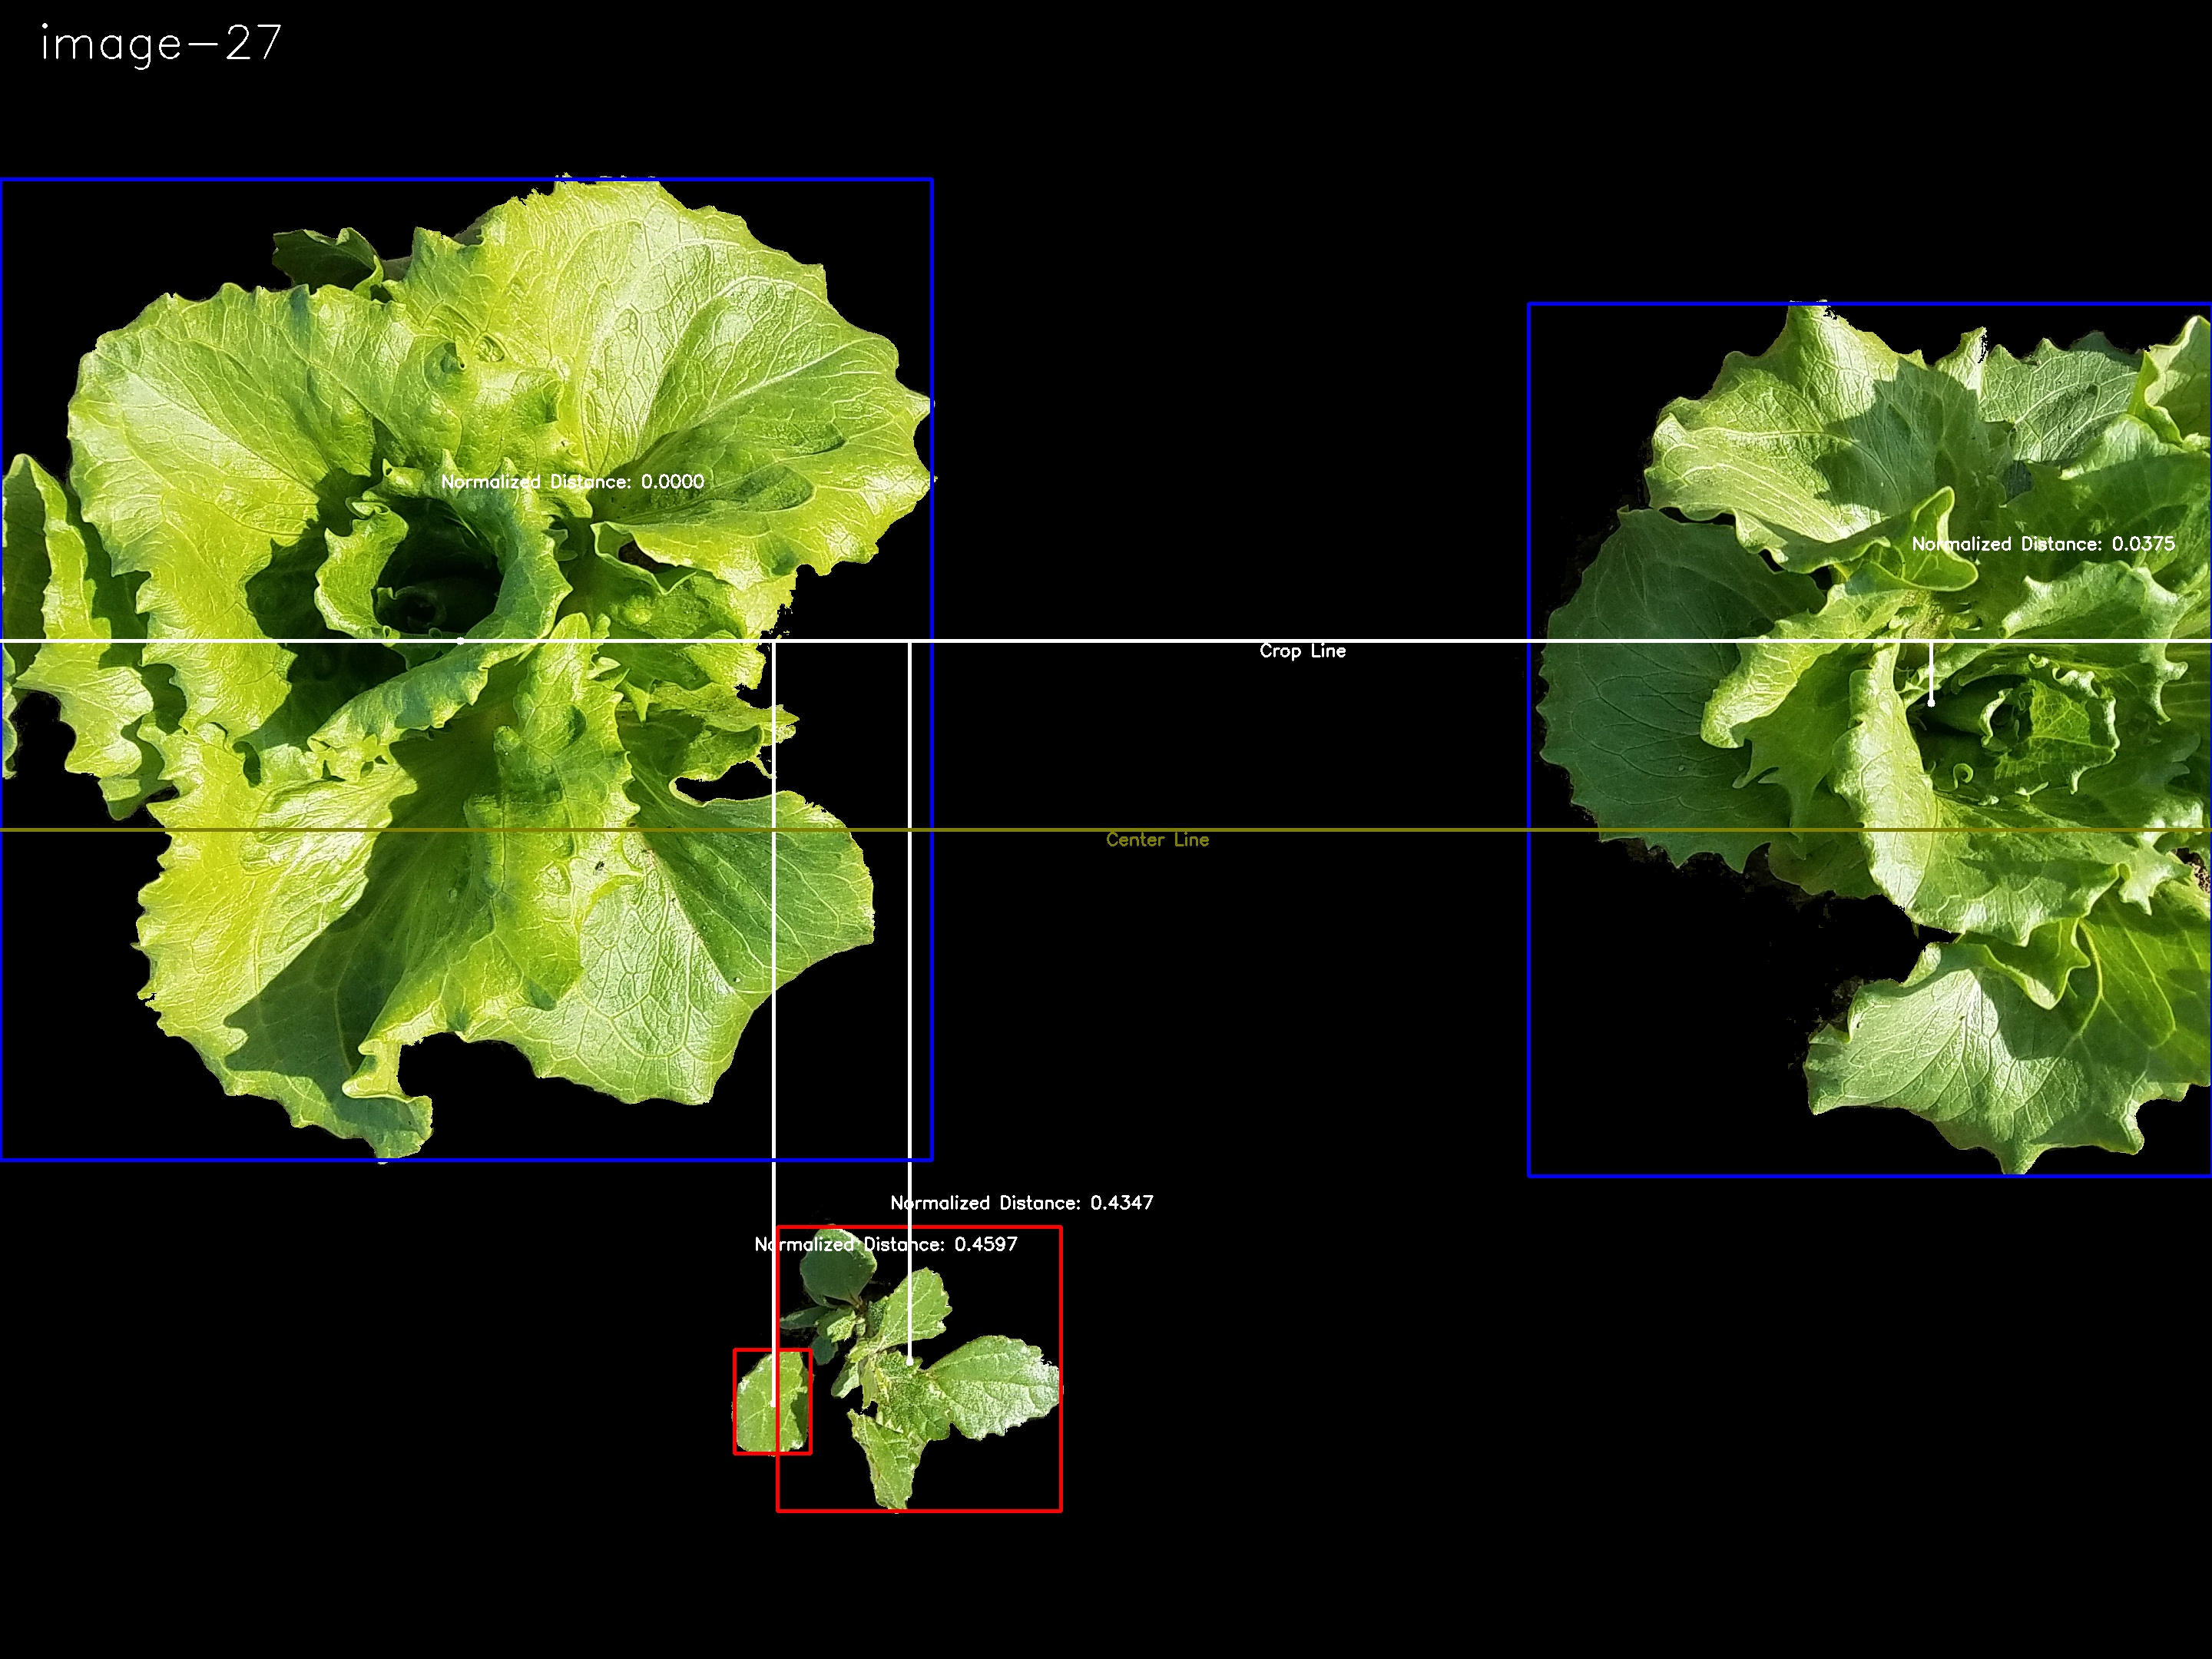
\includegraphics[width=0.4\linewidth]{./figures/normalized-distance.jpg}
	\caption{Normalized Distance to Cropline}
	\label{fig:normalized-distance}
\end{figure}
Figure~\ref{fig:normalized-distance} illustrates the concept of a cropline and the normalized distance of vegetation from it. In this image we see two growths of lettuce that are very close to the cropline (distances here are in pixels, but the units are not significant. This could be expressed in millimeters) at 0 and 0.375 and a weed lying 0.4347 units from the cropline. The values normalized between 0 and 1 by considering the maximum distance the vegetation could be away from the crop line. The line marked {\it Center Line} is for reference purposes and can be ignored for now.  There are two additional items that are worth noting about this image: the dots connecting the plant to the cropline are the {\it centroids} mentioned earlier, and the colored bounding boxes signify the class of the object, something we will return to in a later section.

% H U E
\subsection{Hue}
The terms {\it color} and {\it hue} are often used interchangeably, and while this is mostly true, hue refers to the dominant color family. In this case, the image is converted to the Hue Saturation and Intensity {\it HSV} colorspace and the mean value for the hue is taken.

% S A T U R A T I O N
\subsection{Saturation}
In this case, the image is converted to the Hue Saturation and Intensity {\it HSI} colorspace and the mean value for the saturation is taken. \cite{Various_undated-yv}

\subsection{YIQ}
The YIQ model of color us used by the NTSC color TV system. Y represents the luma information, I and Q the chrominance information. The processing employed here is to convert the image to the YIQ color space and take the mean value for the I, or in-phase component.
\begin{figure}[h!]
	\centering
	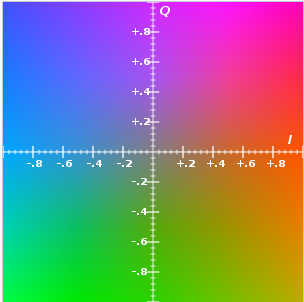
\includegraphics[width=0.4\linewidth]{./figures/yiq.png}
	\caption{YIQ (Reproduced from\protect\cite{Various_undated-cz})}
	\label{fig:yiq}
\end{figure}
The $I$ component is the feature of interest here, and conversion of RGB to YIQ is achieved with this transformation:
\begin{eqnarray*}
	\begin{bmatrix}
	Y \\[0.3em]
	I \\[0.3em]
	Q \\[0.3em]
	\end{bmatrix}
	\approx
	\begin{bmatrix}
	0.299 & 0.587 & 0.114 \\[0.3em]
	0.5959 & -0.2746 & -0.3213\\[0.3em]
	0.2115 & -0.5227 & 0.3112 \\[0.3em]
	\end{bmatrix}
	\begin{bmatrix}
	R \\[0.3em]
	G \\[0.3em]
	B \\[0.3em]
	\end{bmatrix}	
\end{eqnarray*}

\subsection{Compactness}
The compactness of an object is defined as the ratio of its area to the area of a circle with the same perimeter as the original object, and is given by this equation \cite{Wirth2004-li}:
\begin{eqnarray*}
\frac {4 \pi\ area} {perimeter^2}
\end{eqnarray*} 
The most compact object is a circle, whose value is computed as $1$.  Objects with irregular boundaries will have values larger than 1. 
\begin{figure}[H]
	\centering
	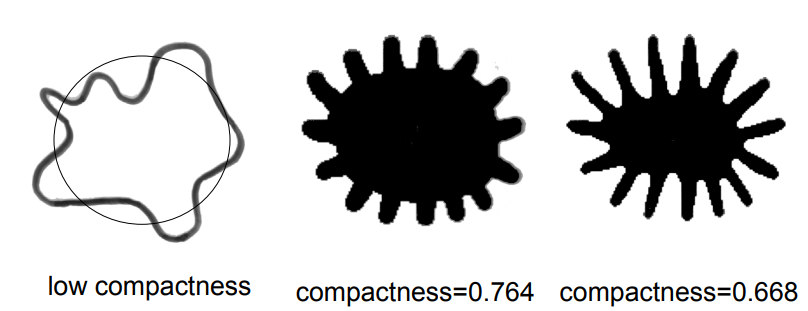
\includegraphics[width=0.4\linewidth]{./figures/compactness.png}
	\caption{Examples of compactness \protect\cite{Wirth2004-li}}
	\label{fig:compactness}
\end{figure}

\subsection{Elongation}
Elongation is the ratio of the length to the width of an object's bounding box \cite{Wirth2004-li}:
\begin{eqnarray*}
\frac {width_{bounding}} {length_{bounding}}
\end{eqnarray*}
This produces a metric between 0 (more elongated) and 1 (roughly circular or square).
\begin{figure}[H]
	\centering
	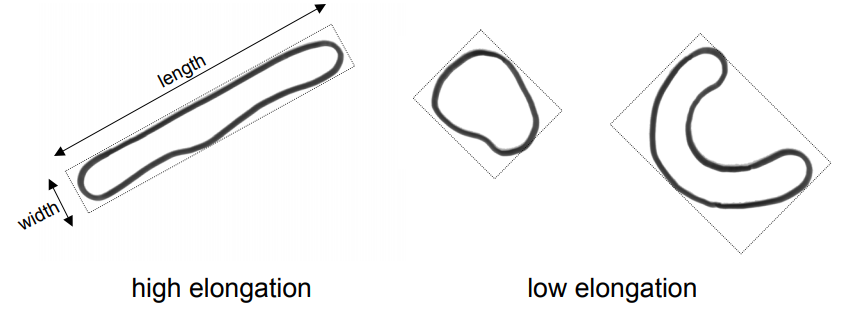
\includegraphics[width=0.4\linewidth]{./figures/elongation.png}
	\caption{Examples of elongation Source: \protect\cite{Wirth2004-li} }
	\label{fig:elongation}
\end{figure}
\subsection{Eccentricity}
The eccentricity (or ellipticity) of an object is the ratio of the length of the minor axis to the length of the major axis. 
\begin{eqnarray*}
\frac {length_{minor-axis}} {length_{major-axis}}
\end{eqnarray*}
The major axis of an object is expressed as the (x,y) endpoints of the longest line that can be drawn through an object. The minor exis is the longest line that can be drawn through an object while remaining perpendicular to the major axis. \cite{Wirth2004-li}
\begin{figure}[H]
	\centering
	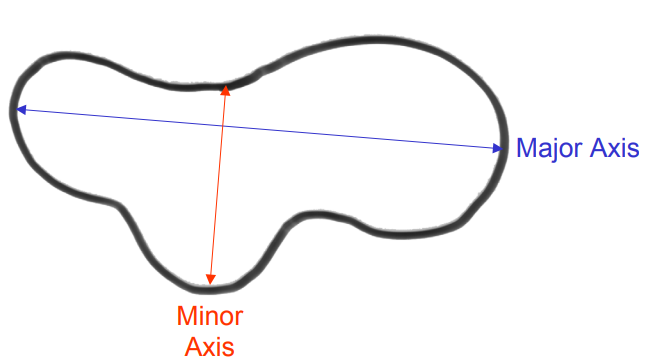
\includegraphics[width=0.4\linewidth]{./figures/major-minor-axis.png}
	\caption{Illustration of major and minor axis \protect\cite{Wirth2004-li} }
	\label{fig:major-minor}
\end{figure}

\subsection{Roundness}
The roundness of an object is an expression varying between 1 (perfectly circular) and 0 (departure from circularity).
\begin{eqnarray*}
\frac {4 \pi\ area} {(convex\ perimeter)^2}
\end{eqnarray*}


\subsection{Convexity}
The convexity of an object is the amount an object differs from a convex object, expressed as the ratio of an object's convex perimeter to the perimeter \cite{Wirth2004-li}:
\begin{eqnarray*}
\frac {convex\ perimeter} {perimeter}
\end{eqnarray*}
\begin{figure}[H]
	\centering
	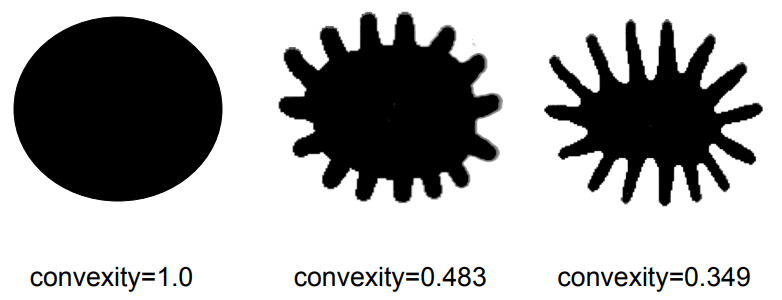
\includegraphics[width=0.4\linewidth]{./figures/convexity.png}
	\caption{Illustration of convexity \protect\cite{Wirth2004-li} }
	\label{fig:convexity}
\end{figure}

\subsection{Solidity}
The solidity of an object varies between 1 (completely solid) and 0, an indication that the object has irregular boundaries.
\begin{eqnarray*}
\frac {area} {convex\ area}
\end{eqnarray*}
\begin{figure}[H]
	\centering
	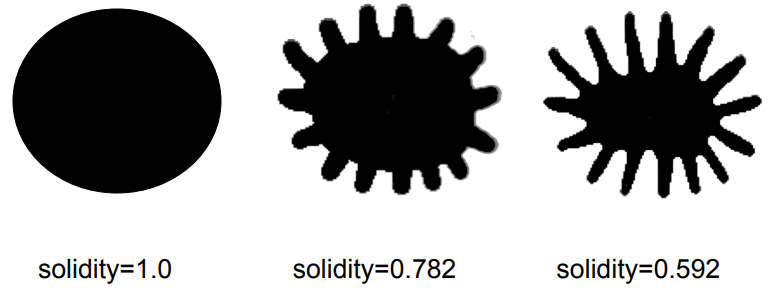
\includegraphics[width=0.4\linewidth]{./figures/solidity.png}
	\caption{Illustration of solidity \protect\cite{Wirth2004-li} }
	\label{fig:solidity}
\end{figure}

\section{Feature Selection}
The features described in the previous section were generated for a set of segmented images, resulting in each object being described by these attributes. Several technique were then used to explore the relationship between these attributes and the labeled class. Specifically, only the most important variables will be selected in the predictions, and those parameters with a weak association will be dropped.
\subsection{Univariate}
In the univariate scheme, the features with the strongest association with the class are selected. In this scheme, scikit-learn supports a suite of statistical tests, and we will use the ANOVA F-value method for feature evaluation. Table~\ref{fig:univariate} shows that the {\it YIQ} feature is, by far, the most interesting feature, and likewise the {\it Eccentricity} the least.

 {
\centering\settowidth\rotheadsize{\bfseries(our proposal)}
\renewcommand\theadalign{cl}\renewcommand\cellalign{cl}
\renewcommand\theadfont{\bfseries}
\renewcommand\tabcolsep{4pt}\renewcommand\arraystretch{1.25}
% Make this a bit smaller so it will fit on a page.  Still looks a bit nasty in that it extends to the edge of the page.
% It's that PCA line that is the trouble, as the values are just too long
\footnotesize
\begin{longtable}[c]{
    |l |*{12}{c |} }%
    \hline
    %\diagbox[height=1.2\rotheadsize, width=\dimexpr\eqboxwidth{AB}+2\tabcolsep\relax]%
    %{\raisebox{1.2ex}{Feature}}{\raisebox{-5ex}{Feature}} &
    {\textbf{Feature}} & {\textbf{ANOVA F-Value}}\\
    %\rothead{Tool X\\\mbox{(our proposal)}}\\
    \hline
    \eqmakebox{Length-Width Ratio} & 24.575 \\
    \eqmakebox{Shape Index} & 120.546 \\
    \eqmakebox{Distance} &  70.1 \\
    \eqmakebox{Normalized Distance} & 138.479  \\
    \eqmakebox{Hue} & 1.124  \\
    \eqmakebox{Saturation} & 134.901  \\
    \eqmakebox{YIQ Mean} & 517.799 \\
    \eqmakebox{Compactness} & 115.005  \\
    \eqmakebox{Eccentricity} & 0.321 \\
    \eqmakebox{Roundness} & 38.047  \\
    \eqmakebox{Convexity} & 1.041  \\
    \eqmakebox{Solidity} & 34.082 \\
    \hline
    \caption{Univariate Feature Selection}
    \label{fig:univariate}
  \end{longtable}
 }
%\subsection{Low Variance}
\subsection{Feature Importance}
The Feature Importance scheme uses Random Forest and Extra Trees approaches to rank features for importance.

Applying this to the dataset created results in these scores, where more important features are assigned higher scores. Table~\ref{fig:importance} shows the results of the scores assigned to the various features.   In this table, we can see that the {\it YIQ}, the {\it Normalized Distance}, and the {\it Compactness} are the most important features. Interestingly, color features play prominently here, far exceeding the scores assigned to structural features such as the {\it Solidity} of an object. Structural features such as {\it Eccentricity} have scores low enough that it is likely the case that they could be omitted from the model without a negative impact on accuracy.

{
\centering\settowidth\rotheadsize{\bfseries(our proposal)}
\renewcommand\theadalign{cl}\renewcommand\cellalign{cl}
\renewcommand\theadfont{\bfseries}
\renewcommand\tabcolsep{4pt}\renewcommand\arraystretch{1.25}
% Make this a bit smaller so it will fit on a page.  Still looks a bit nasty in that it extends to the edge of the page.
% It's that PCA line that is the trouble, as the values are just too long
\footnotesize
\begin{longtable}[c]{
    |l |*{12}{c |} }%
    \hline
    %\diagbox[height=1.2\rotheadsize, width=\dimexpr\eqboxwidth{AB}+2\tabcolsep\relax]%
    %{\raisebox{1.2ex}{Feature}}{\raisebox{-5ex}{Feature}} &
    {\textbf{Feature}} & {\textbf{Importance Score}}\\
    %\rothead{Tool X\\\mbox{(our proposal)}}\\
    \hline
    \eqmakebox{Length-Width Ratio} & 0.02998853 \\
    \eqmakebox{Shape Index} & 0.05357191 \\
    \eqmakebox{Distance} &  0.05081641 \\
    \eqmakebox{Normalized Distance} & 0.12969820 \\
    \eqmakebox{Hue} & 0.00542753  \\
    \eqmakebox{Saturation} & 0.08911404  \\
    \eqmakebox{YIQ Mean} & 0.38947503  \\
    \eqmakebox{Compactness} & 0.09122537  \\
    \eqmakebox{Eccentricity} & 0.00761004 \\
    \eqmakebox{Roundness} & 0.04467927  \\
    \eqmakebox{Convexity} & 0.05499904   \\
    \eqmakebox{Solidity} & 0.05339462  \\
    \hline
    \caption{Feature Importance Scores}
    \label{fig:importance}
  \end{longtable}
 }
\subsubsection{Implementation Details}
The feature importances were evaluated using the {\it ExtraTreesClassifier} from scikit-learn:

\begin{lstlisting}
        model = ExtraTreesClassifier(n_estimators=10)
        model.fit(x, y)
        print(model.feature_importances_)
\end{lstlisting}

 
\subsection{Recursive Elimination}
The Recursive Feature Elimination scheme works backwards from a full model (all attributes) to remove attributes, build a model, and evaluate the results to characterize a feature's contribution to the prediction. Table~\ref{fig:recursive} shows an unexpected result.  While {\it Normalized Distance} is, once again,  an important feature, {\it YIQ} is now near the bottom of the list.

{
\centering\settowidth\rotheadsize{\bfseries(our proposal)}
\renewcommand\theadalign{cl}\renewcommand\cellalign{cl}
\renewcommand\theadfont{\bfseries}
\renewcommand\tabcolsep{4pt}\renewcommand\arraystretch{1.25}
% Make this a bit smaller so it will fit on a page.  Still looks a bit nasty in that it extends to the edge of the page.
% It's that PCA line that is the trouble, as the values are just too long
\footnotesize
\begin{longtable}[c]{
    |l |*{12}{c |} }%
    \hline
    %\diagbox[height=1.2\rotheadsize, width=\dimexpr\eqboxwidth{AB}+2\tabcolsep\relax]%
    %{\raisebox{1.2ex}{Feature}}{\raisebox{-5ex}{Feature}} &
    {\textbf{Feature}} & {\textbf{Importance Rank}}\\
    %\rothead{Tool X\\\mbox{(our proposal)}}\\
    \hline
    \eqmakebox{Length-Width Ratio} & 3 \\
    \eqmakebox{Shape Index} & 2 \\
    \eqmakebox{Distance} &  12 \\
    \eqmakebox{Normalized Distance} & 1  \\
    \eqmakebox{Hue} & 9  \\
    \eqmakebox{Saturation} & 10  \\
    \eqmakebox{YIQ Mean} & 11  \\
    \eqmakebox{Compactness} & 4  \\
    \eqmakebox{Eccentricity} & 7 \\
    \eqmakebox{Roundness} & 5  \\
    \eqmakebox{Convexity} & 8  \\
    \eqmakebox{Solidity} & 6  \\
    \hline
    \caption{Feature Importance Ranks using RFE with a Logistic Regression Classifier}
    \label{fig:recursive}
  \end{longtable}
 }
 
 As noted in the introduction, this is not a balanced dataset, as the weed class is underrepresented. Adjusting the weights a bit by an arbitrary amount (0.8 crop, 0.2 weeds) yields a quite different result, as illustrated in Table~\ref{fig:recursive-weighted}. Here, note that the {\it YIQ} parameter is dramatically different, appearing as the $7^{th}$ most important parameter now.
 
 {
\centering\settowidth\rotheadsize{\bfseries(our proposal)}
\renewcommand\theadalign{cl}\renewcommand\cellalign{cl}
\renewcommand\theadfont{\bfseries}
\renewcommand\tabcolsep{4pt}\renewcommand\arraystretch{1.25}
% Make this a bit smaller so it will fit on a page.  Still looks a bit nasty in that it extends to the edge of the page.
% It's that PCA line that is the trouble, as the values are just too long
\footnotesize
\begin{longtable}[c]{
    |l |*{12}{c |} }%
    \hline
    %\diagbox[height=1.2\rotheadsize, width=\dimexpr\eqboxwidth{AB}+2\tabcolsep\relax]%
    %{\raisebox{1.2ex}{Feature}}{\raisebox{-5ex}{Feature}} &
    {\textbf{Feature}} & {\textbf{Importance Rank}}\\
    %\rothead{Tool X\\\mbox{(our proposal)}}\\
    \hline
    \eqmakebox{Length-Width Ratio} & 2 \\
    \eqmakebox{Shape Index} & 1 \\
    \eqmakebox{Distance} &  12 \\
    \eqmakebox{Normalized Distance} & 3  \\
    \eqmakebox{Hue} & 11  \\
    \eqmakebox{Saturation} & 10  \\
    \eqmakebox{YIQ Mean} & 7  \\
    \eqmakebox{Compactness} & 4  \\
    \eqmakebox{Eccentricity} & 6 \\
    \eqmakebox{Roundness} & 5  \\
    \eqmakebox{Convexity} & 8  \\
    \eqmakebox{Solidity} & 9  \\
    \hline
    \caption{Feature Importance Ranks using RFE with a Logistic Regression Classifier with weighted classes}
    \label{fig:recursive-weighted}
  \end{longtable}
 }
 
 Using a random forest classifier changes the picture yet again. As Table~\ref{fig:random-forest} shows, {\it YIQ} is now the most important feature to consider.
 
{
\centering\settowidth\rotheadsize{\bfseries(our proposal)}
\renewcommand\theadalign{cl}\renewcommand\cellalign{cl}
\renewcommand\theadfont{\bfseries}
\renewcommand\tabcolsep{4pt}\renewcommand\arraystretch{1.25}
% Make this a bit smaller so it will fit on a page.  Still looks a bit nasty in that it extends to the edge of the page.
% It's that PCA line that is the trouble, as the values are just too long
\footnotesize
\begin{longtable}[c]{
    |l |*{12}{c |} }%
    \hline
    %\diagbox[height=1.2\rotheadsize, width=\dimexpr\eqboxwidth{AB}+2\tabcolsep\relax]%
    %{\raisebox{1.2ex}{Feature}}{\raisebox{-5ex}{Feature}} &
    {\textbf{Feature}} & {\textbf{Importance Rank}}\\
    %\rothead{Tool X\\\mbox{(our proposal)}}\\
    \hline
    \eqmakebox{Length-Width Ratio} & 7 \\
    \eqmakebox{Shape Index} & 6 \\
    \eqmakebox{Distance} &  8 \\
    \eqmakebox{Normalized Distance} & 3  \\
    \eqmakebox{Hue} & 11  \\
    \eqmakebox{Saturation} & 2  \\
    \eqmakebox{YIQ Mean} & 1  \\
    \eqmakebox{Compactness} & 4  \\
    \eqmakebox{Eccentricity} & 12 \\
    \eqmakebox{Roundness} & 5  \\
    \eqmakebox{Convexity} & 10  \\
    \eqmakebox{Solidity} & 9  \\
    \hline
    \caption{Feature Importance Ranks using RFE with a Random Forest Classifier}
    \label{fig:random-forest}
  \end{longtable}
 }
 \subsubsection{Implementation Details}
The feature importance was evaluated using the {\it LogisticRegression} and {\it RandomForestClassifier} class from scikit-learn:

\begin{lstlisting}
        features = self._rawData.values
        # x is everything
        # y is just the type
        x = features[:,0:self._rawData.shape[1]-1]
        y = features[:,self._rawData.shape[1]-1]
        weights = {0: 0.8, 1: 0.2}
        #model = LogisticRegression(solver='lbfgs', max_iter=200)
        #model = LogisticRegression(solver='liblinear', class_weight=weights, max_iter=200)
        model = RandomForestClassifier(n_estimators=100, random_state=42)
        rfe = RFE(model, n_features_to_select=1)
        fit = rfe.fit(x, y)
        print("Num Features: %d" % fit.n_features_)
        print("Selected Features: %s" % fit.support_)
        print("Feature Ranking: %s" % fit.ranking_)
\end{lstlisting}

 
\subsection{Principal Component Analysis}
Principal Component Analysis (PCA) involves re-projecting the data (a change in basis) as a technique to reduce the dimensionality of the data \cite{Muller2016-ui}.  In Figure~\ref{fig:pca} we see that most of the variance can be explained by only 3 features: {\it Length-Width Ratio}, {\it Shape Index}, and {\it Distance}.
\begin{figure}[H]
\centering
\begin{subfigure}[]{.32\textwidth}
	  \centering
	  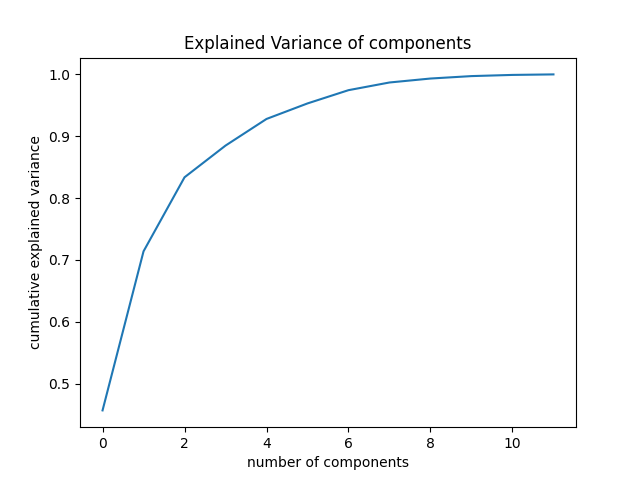
\includegraphics[width=1\linewidth]{figures/explained-variance}
	  \caption{Features explaining variance}
	  %\label{fig:sub1}
\end{subfigure}
\begin{subfigure}{.32\textwidth}
  \centering
	{
	\centering\settowidth\rotheadsize{\bfseries(our proposal)}
	\renewcommand\theadalign{cl}\renewcommand\cellalign{cl}
	\renewcommand\theadfont{\bfseries}
	\renewcommand\tabcolsep{4pt}\renewcommand\arraystretch{1.25}
	% Make this a bit smaller so it will fit on a page.  Still looks a bit nasty in that it extends to the edge of the page.
	% It's that PCA line that is the trouble, as the values are just too long
	\footnotesize
	\begin{longtable}[c]{
	    |l |*{12}{c |} }%
	    \hline
	    %\diagbox[height=1.2\rotheadsize, width=\dimexpr\eqboxwidth{AB}+2\tabcolsep\relax]%
	    %{\raisebox{1.2ex}{Feature}}{\raisebox{-5ex}{Feature}} &
	    {\textbf{Feature}} & {\textbf{Importance Rank}}\\
	    %\rothead{Tool X\\\mbox{(our proposal)}}\\
	    \hline
	    \eqmakebox{Length-Width Ratio} & 9.85653384e-01 \\
	    \eqmakebox{Shape Index} & 1.32174325e-02 \\
	    \eqmakebox{Distance} &  1.10130275e-03  \\
	    \eqmakebox{Normalized Distance} & 2.48181154e-05  \\
	    \eqmakebox{Hue} & 1.72566121e-06   \\
	    \eqmakebox{Saturation} & 1.09271410e-06   \\
	    \eqmakebox{YIQ Mean} & 1.62825386e-07  \\
	    \eqmakebox{Compactness} & 3.91351740e-08  \\
	    \eqmakebox{Eccentricity} & 2.61087301e-08 \\
	    \eqmakebox{Roundness} & 1.26245056e-08  \\
	    \eqmakebox{Convexity} & 3.39049614e-09  \\
	    \eqmakebox{Solidity} & 3.55200370e-10  \\
	    \hline
	    %\caption{Feature Importance Ranks using RFE with a Random Forest Classifier}
	    %\label{fig:random-forest}
	  \end{longtable}
	 }
  \caption{PCA Variances}
  %\label{fig:sub2}
\end{subfigure}
\caption{Principal Component Analysis of Features}
\label{fig:pca}
\end{figure}

\subsubsection{Implementation Details}
The principal component analysis was evaluated using the {\it PCA} class from scikit-learn:

\begin{lstlisting}
        features = self._rawData.values
        # x is everything
        # y is just the type
        x = features[:,0:self._rawData.shape[1]-1]
        y = features[:,self._rawData.shape[1]-1]
        pca = PCA(n_components=12)
        fit = pca.fit(x)
        print("Explained Variance: %s" % fit.explained_variance_ratio_)
        print(fit.components_)
\end{lstlisting}

\subsection{Feature Selections}

Table~\ref{fig:highlighted-selections} shows a summary of various approaches with the top 3 features highlighted. Unfortunately, the results are not completely consistent across the various approaches. There are a few themes, however:
\begin{itemize}
\item{Aspects of color data are quite predictive in the YIQ and HSI color spaces. More investigation on color space is needed}
\item{Most structural attributes (convexity, roundness, etc) are not significant.}
\item{Placement within a crop row is one of the more consistent attributes, and this is not entirely surprising. A crop most often falls near a cropline, and weeds most often away from the crop line}
\end{itemize}



% Put the table in its own object
{
\centering\settowidth\rotheadsize{\bfseries(our proposal)}
\renewcommand\theadalign{cl}\renewcommand\cellalign{cl}
\renewcommand\theadfont{\bfseries}
\renewcommand\tabcolsep{4pt}\renewcommand\arraystretch{1.25}
% Make this a bit smaller so it will fit on a page.  Still looks a bit nasty in that it extends to the edge of the page.
% It's that PCA line that is the trouble, as the values are just too long
% Make the color blue for the top three features in each category
\footnotesize
\begin{longtable}{
    |l |*{12}{c |} }%
    \hline
    \diagbox[height=1.2\rotheadsize, width=\dimexpr\eqboxwidth{AB}+2\tabcolsep\relax]%
    {\raisebox{1.2ex}{Selection}}{\raisebox{-5ex}{Feature}} &
    \rotcell{Length-Width Ratio} &
    \rotcell{Shape Index} &
    \rotcell{Distance} &
    \rotcell{Normalized Distance} &
    \rotcell{Hue} &
    \rotcell{Saturation} &
    \rotcell{YIQ Mean} &
    \rotcell{Compactness} &
    \rotcell{Eccentricity} &
    \rotcell{Roundness} &
    \rotcell{Convexity} &
    \rotcell{Solidity}\\
    %\rothead{Tool X\\\mbox{(our proposal)}}\\
    \hline
    \eqmakebox[AB][l]{Univariate} & 23.6 & 120.5 & 70.1 & \cellcolor{blue!25} 138.6 & 1.1 & \cellcolor{blue!25} 134.9 & \cellcolor{blue!25} 517.8 & 115.0 & 0.3 & 38.0 & 1.0 & 34.1 \\
    %\eqmakebox[AB]{Variance} & 2.114 & 0.008 & 9150.389 & 0.027 & 117.093 & 1350.474 & $>$0.001 & 0.0376 & 0.174 & 0.174 & 0.312 & 0.014 \\
    % Not sure why these come out centered and the first two are left aligned.
    \eqmakebox[AB]{Recursive} &\cellcolor{blue!25} 3  &\cellcolor{blue!25} 2 &12  &\cellcolor{blue!25} 1  &9 &10 &11  &4  &7  &5  &8  &6 \\
    %\eqmakebox[AB]{PCA} & 9.85e-01 & 1.32e-02 & 1.10e-03 & 2.48e-05 & 1.726e-06 & 1.093e-06 & 1.63e-07 & 3.91e-08 & 2.61e-08 & 1.26e-08 & 3.39e-09 & 3.55e-10\\
    % Rounding off the values makes this fit.
    \eqmakebox[AB]{PCA} &\cellcolor{blue!25} 9.9e-01 & \cellcolor{blue!25} 1.3e-02 & \cellcolor{blue!25} 1.1e-03 & 2.5e-05 & 1.7e-06 & 1.1e-06 & 1.6e-07 & 3.9e-08 & 2.6e-08 & 1.3e-08 & 3.4e-09 & 3.6e-10\\
    \eqmakebox[AB]{Importance} &0.039  &0.070 &0.027 &\cellcolor{blue!25} 0.260 &0.033 &\cellcolor{blue!25} 0.108 &\cellcolor{blue!25} 0.252 &0.087 &0.015 &0.067 &0.011  &0.032\\
    \hline
    \caption{Feature Selection using various approaches.}
    \label{fig:highlighted-selections}
  \end{longtable}
 }
 
  Given these observations, we can use these parameters for our training and prediction:
 \begin{itemize}
	\item{The length/width ratio}
	\item{The shape index}
	\item{The YIQ in-phase mean}
	\item{The Normalized distance from the cropline}
\end{itemize}
  
  
\section{Crop/Weed Discrimination}

Using the subset of the parameters identified in the previous section, various approaches were used in classifying the objects isolated in the images and detailed in Table~\ref{fig:learning}.

{\renewcommand{\arraystretch}{2}%
\begin{table}[H]
	\centering
    \caption{Learning Results}
    \label{fig:learning}
    \begin{tabular}{  l  p{4cm}  p{5cm} }
     %\begin{tabular}{  l  p{3.4cm}  p{3.4cm} }
        \toprule
\textbf{Method}      
& \textbf{Train}   
& \textbf{Test} \\\midrule
Logistic Regression
& 0.9790       
& 0.9787 \\\hline
KNN     
& $1.0$                    
& $0.86$ \\\hline
Decision Tree
& 1.0
& 0.96 \\\hline
Boosted Gradient     
& 1.0
& 0.957 \\\hline
Random Forest      
& 1.0
& 0.986 \\\hline
    
        \bottomrule
    \end{tabular}
\end{table}

For this sample dataset, all approaches with the exception of KNN yield commercially acceptable results if accuracy were the only criterion used in evaluation. However this case must consider two other criteria that are important, but beyond the scope of this document:
\begin{itemize}
\item{The computational cost of achieving each result. The prediction will be done in real-time under field conditions\footnote{And on a GPU, not on a CPU as was done here} While a result of an approach yielding results above 98\% may sound impressive, if that prediction using logistic regression takes a few hundred milliseconds and a decision tree takes well under 100 milliseconds, it may be the case that using that logistic regression in practice is not viable.\footnote{Some context is probably needed here. This prediction will be done as a tractor is moving along, and the time spent on prediction is part of an overall time budget that will ultimately limit the forward speed of the tractor. 2 MPH is commercially viable. 1 MPH is not.}}
\item{The cost of classifying a crop as a weed has very real dollar cost, as the subsequent killing of that plant would negatively impact the farmer. The cost of classifying a weed as a crop (and thus not flagging it for treatment) is much lower. While it may have modest financial impact, as leaving the weed in place allows it to take resources away from marketable vegetation (water, fertilizer), the impact of doing so may be acceptable in most instances.}
\end{itemize}
 
Figure~\ref{fig:classified} shows an annotated classification result.\footnote{In the production field system, of course, images like this will never be used.  This is just so humans can tell what the system is doing.} In this figure, we see desirable (crop) bounded by a green box, and undesirable (not crop) bounded in red. The blue box bounds vegetation for which we can't reliably determine its class. Computations that depend on an unimpeded view of the vegetation ({\it length/width ratio}, for instance) can't be reliably performed. Some color computations could be, but may not be as representative as required. The {\it hue} value, for example, is the mean value across the entire plant, and the hue may not be consistent across the entire plant. The portion that is visible may not be representative of the plant as a whole.

\begin{figure}[H]
	\centering
	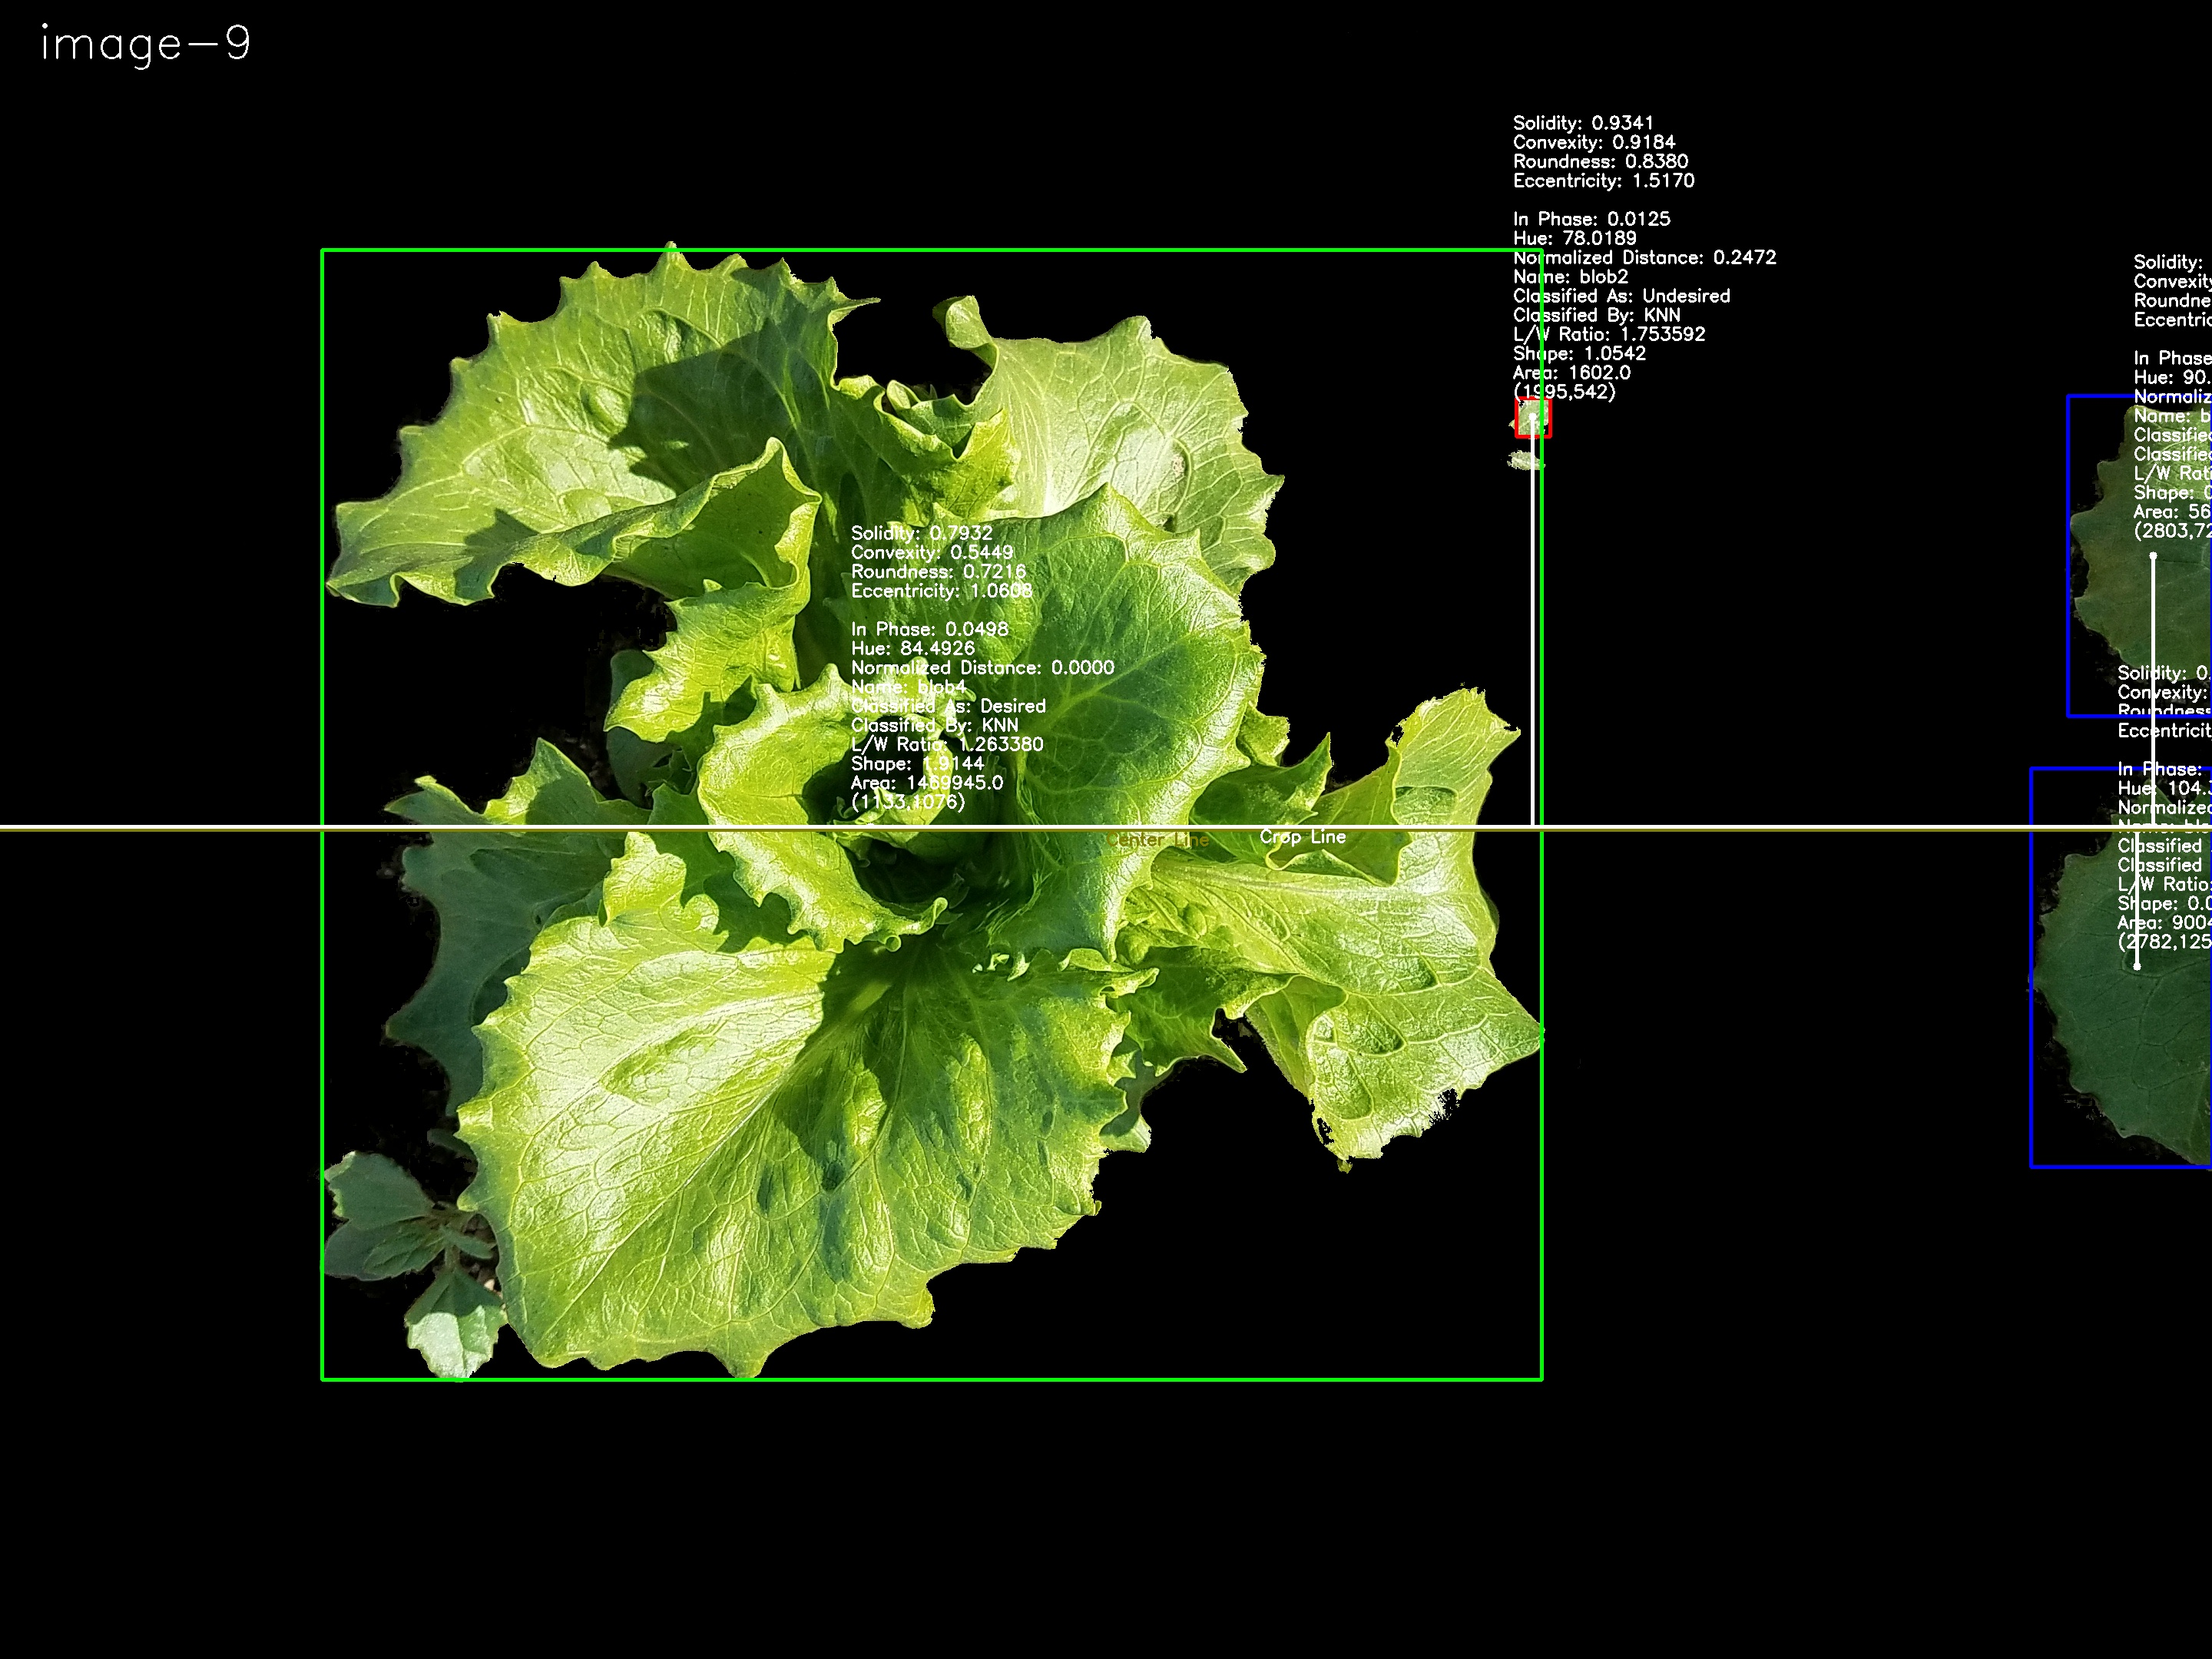
\includegraphics[width=0.7\linewidth]{./figures/classified-result.jpg}
	\caption{A classified result. Desirable vegetation is bounded in green and undesirable in red}
	\label{fig:classified}
\end{figure}

\newpage
\section{References}
\printbibliography[heading=none]

%\cite{Wirth2004-li}
\end{document}

